\documentclass[11pt]{article}
\usepackage[utf8]{inputenc}
\usepackage[spanish]{babel}
\decimalpoint
\usepackage{amsmath}
\usepackage{amsthm}
\usepackage{amssymb}
\usepackage{graphicx}
\usepackage[margin=0.8in]{geometry}
\usepackage{fancyhdr}
\usepackage[inline]{enumitem}
\usepackage{float}
\usepackage{cancel}
\usepackage{bigints}
\usepackage{listings}
\usepackage{xcolor}
\usepackage{listingsutf8}
\usepackage{algpseudocode}
\usepackage{algorithm}
\usepackage{apacite}
\usepackage{tcolorbox}
\usepackage{multicol}
\usepackage{tipa}
\usepackage{caption} 
\pagestyle{fancy}
\usepackage{hyperref}
\usepackage{mathtools}% http://ctan.org/pkg/mathtools

\hypersetup{
    colorlinks,
    citecolor=black,
    filecolor=black,
    linkcolor=black,
    urlcolor=black
}
\newcommand{\xvdash}[1]{%
	\vdash^{\mkern-10mu\scriptscriptstyle\rule[-.9ex]{0pt}{0pt}#1}%
}
\setlength{\headheight}{15pt} 
\lhead{Tarea 3. Multiplicación de matrices distribuida utilizando paso de mensajes}
\rhead{\thepage}
\lfoot{ESCOM-IPN}
\renewcommand{\footrulewidth}{0.5pt}
\setlength{\parskip}{0.5em}
\newcommand{\ve}[1]{\overrightarrow{#1}}
\newcommand{\abs}[1]{\left\lvert #1 \right\lvert}
\newcommand{\blank}{\text{\textcrb}}
\date{\today}
\title{Tarea 3. Multiplicación de matrices distribuida utilizando paso de mensajes}
\author{Sanchez Mendez Edmundo Josue}

\lstset{
tabsize = 4, %% set tab space width
showstringspaces = false, %% prevent space marking in strings, string is defined as the text that is generally printed directly to the console
numbers = left, %% display line numbers on the left
commentstyle = \color{green}, %% set comment color
keywordstyle = \color{blue}, %% set keyword color
stringstyle = \color{red}, %% set string color
rulecolor = \color{black}, %% set frame color to avoid being affected by text color
basicstyle = \small \ttfamily , %% set listing font and size
breaklines = true, %% enable line breaking
numberstyle = \tiny,
}

\bibliographystyle{apacite}
\begin{document}
		\begin{titlepage}
			\begin{center}
				
				% Upper part of the page. The '~' is needed because \\
				% only works if a paragraph has started.
				
				\noindent
				\begin{minipage}{0.5\textwidth}
					\begin{flushleft} \large
						
\includegraphics[width=0.5\textwidth]{resources/ipn.png}
					\end{flushleft}
				\end{minipage}%
				\begin{minipage}{0.55\textwidth}
					\begin{flushright} \large
						
\includegraphics[width=0.5\textwidth]{resources/escom.png}
					\end{flushright}
				\end{minipage}
				
				\textsc{\LARGE Instituto Politécnico Nacional}\\[0.5cm]
				
				\textsc{\Large Escuela Superior de Cómputo}\\[1cm]
				
				% Title
				
				{ \huge Tarea 5. Multiplicación de matrices utilizando objetos distribuidos \\[1cm] }
				
				{ \Large Unidad de aprendizaje: Desarrollo de Sistemas Distribuidos} \\[1cm]
				
				{ \Large Grupo: 4CV11 } \\[1cm]
				
				\noindent
				\begin{minipage}{0.5\textwidth}
					\begin{flushleft} \large
						\emph{Alumno:} \\
						Sanchez Mendez Edmundo Josue
					\end{flushleft}
				\end{minipage}%
				\begin{minipage}{0.5\textwidth}
					\begin{flushright} \large
						\emph{Profesor:} \\
						Pineda Guerrero Carlos 
					\end{flushright}
				\end{minipage}
				
				\vfill
				% Bottom of the page
				{\large {\today}}
			\end{center}
		\end{titlepage}
	
	\titlepage
	\tableofcontents
	\newpage
	
	\section{Introducción}
		Se deberá desarrollar un sistema que calcule el producto de dos matrices cuadradas utilizando Java RMI, tal como fue explicado en clase. Se deberán ejecutar dos casos con las siguientes restricciones:
		\begin{itemize}
			\item N=9, se deberá desplegar las matrices A, B y C y el checksum de la matriz C.
			\item N=3000, deberá desplegar el checksum de la matriz C.
		\end{itemize}
		Recordar que el checksum de la matriz es la suma de los valores de esta. Los requisitos son los siguientes:
		\begin{itemize}
			\item Los elementos de las matrices A, B y C serán de tipo double y el checksum será de tipo double.
			\item Se deberá inicializar las matrices A y B de la siguiente manera:
				\begin{itemize}
					\item A[i][j]= i + 4 * j
					\item B[i][j] = i - 4 * j
				\end{itemize}
			\item Se deberá dividir las matrices A y B en tres partes, por tanto la matriz C estará dividida en 9 partes.
			\item El cliente RMI ejecutará en una máquina virtual con Ubuntu en Azure (nodo 0). El servidor RMI ejecutará en tres máquinas virtuales (nodo 1, nodo 2 y nodo 3) con Ubuntu en Azure. El programa rmiregistry ejecutará en cada nodo donde ejecute el servidor RMI. El nodo 1 calculará los productos C1, C2 y C3, el nodo 2 calculará los productos C4, C5 y C6, y el nodo 3 calculará los productos C7, C8 y C9.
		\end{itemize}
	\section{Desarrollo}
Para el desarrollo de la practica nos basamos en el código dado en clase sobre el calculo de las matrices el cual calcula la multiplicación de las matrices pero las divide en dos partes, un objetivo de la practica es poder dividir las matrices en 3 partes, esto provoca que el resultado sea compuesto por 9 matrices de tamaño N/3 cada una, ademas trae como consecuencia que solo podamos multiplicar matrices de un tamaño múltiplo de 3 para tener un correcto funcionamiento. Después el objetivo final es llevar acabo la multiplicación de las matrices mediante el uso de Java RMI para esto primeramente deberemos crear 4 maquinas virtuales con Java instalado y el código del programa, mencionar que para los nodos 1, 2 y 3 solo necesitamos los archivos ServidorRMI.java, InterfaceRMI.java y Clase.java también en estos nodos debemos iniciar el comando rmiregistry para que la practica funcione, para el nodo 0 solo necesitamos las clases ClienteRMI.java y InterfaceRMI.java.
		\begin{figure}[H]
			\centering
			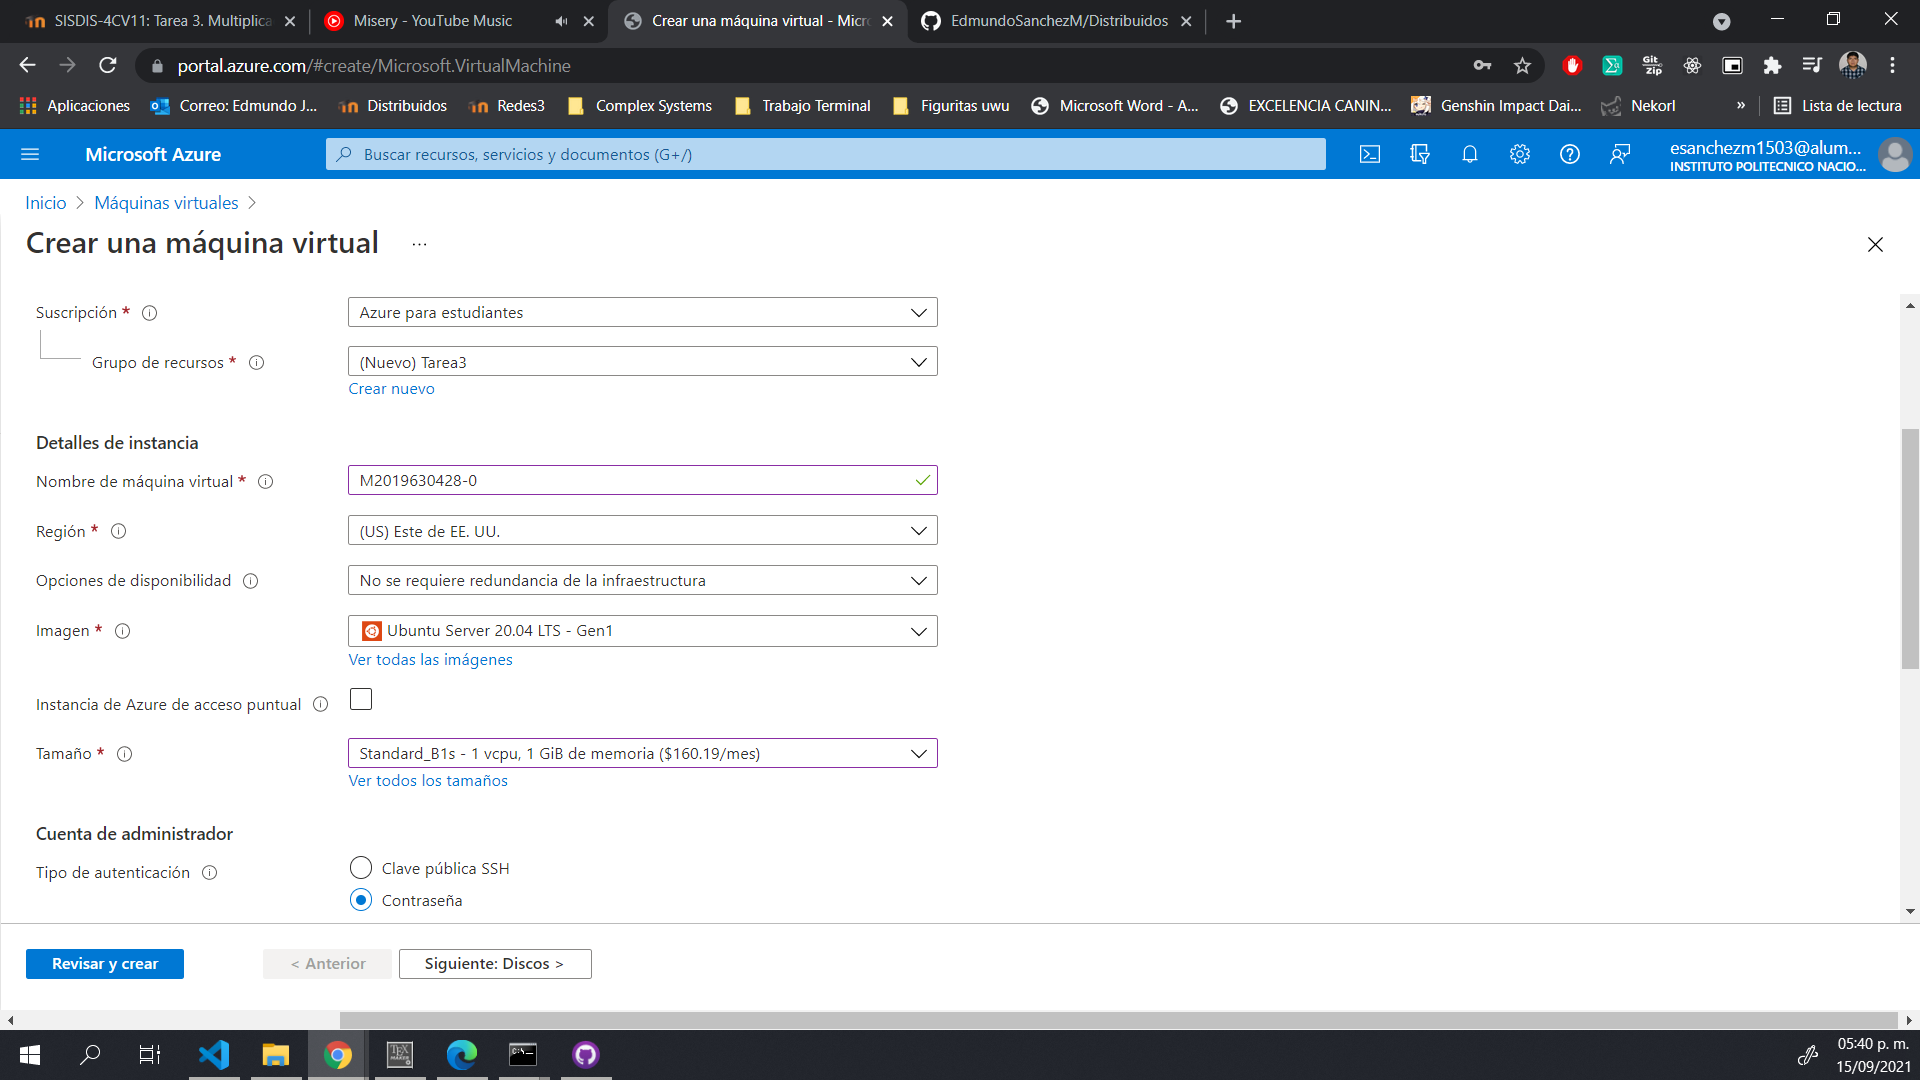
\includegraphics[scale=0.34]{resources/datosbasicos.png}
			\caption{Datos básicos para el nodo 0. }\label{fig:picture}
		\end{figure}
		\begin{figure}[H]
			\centering
			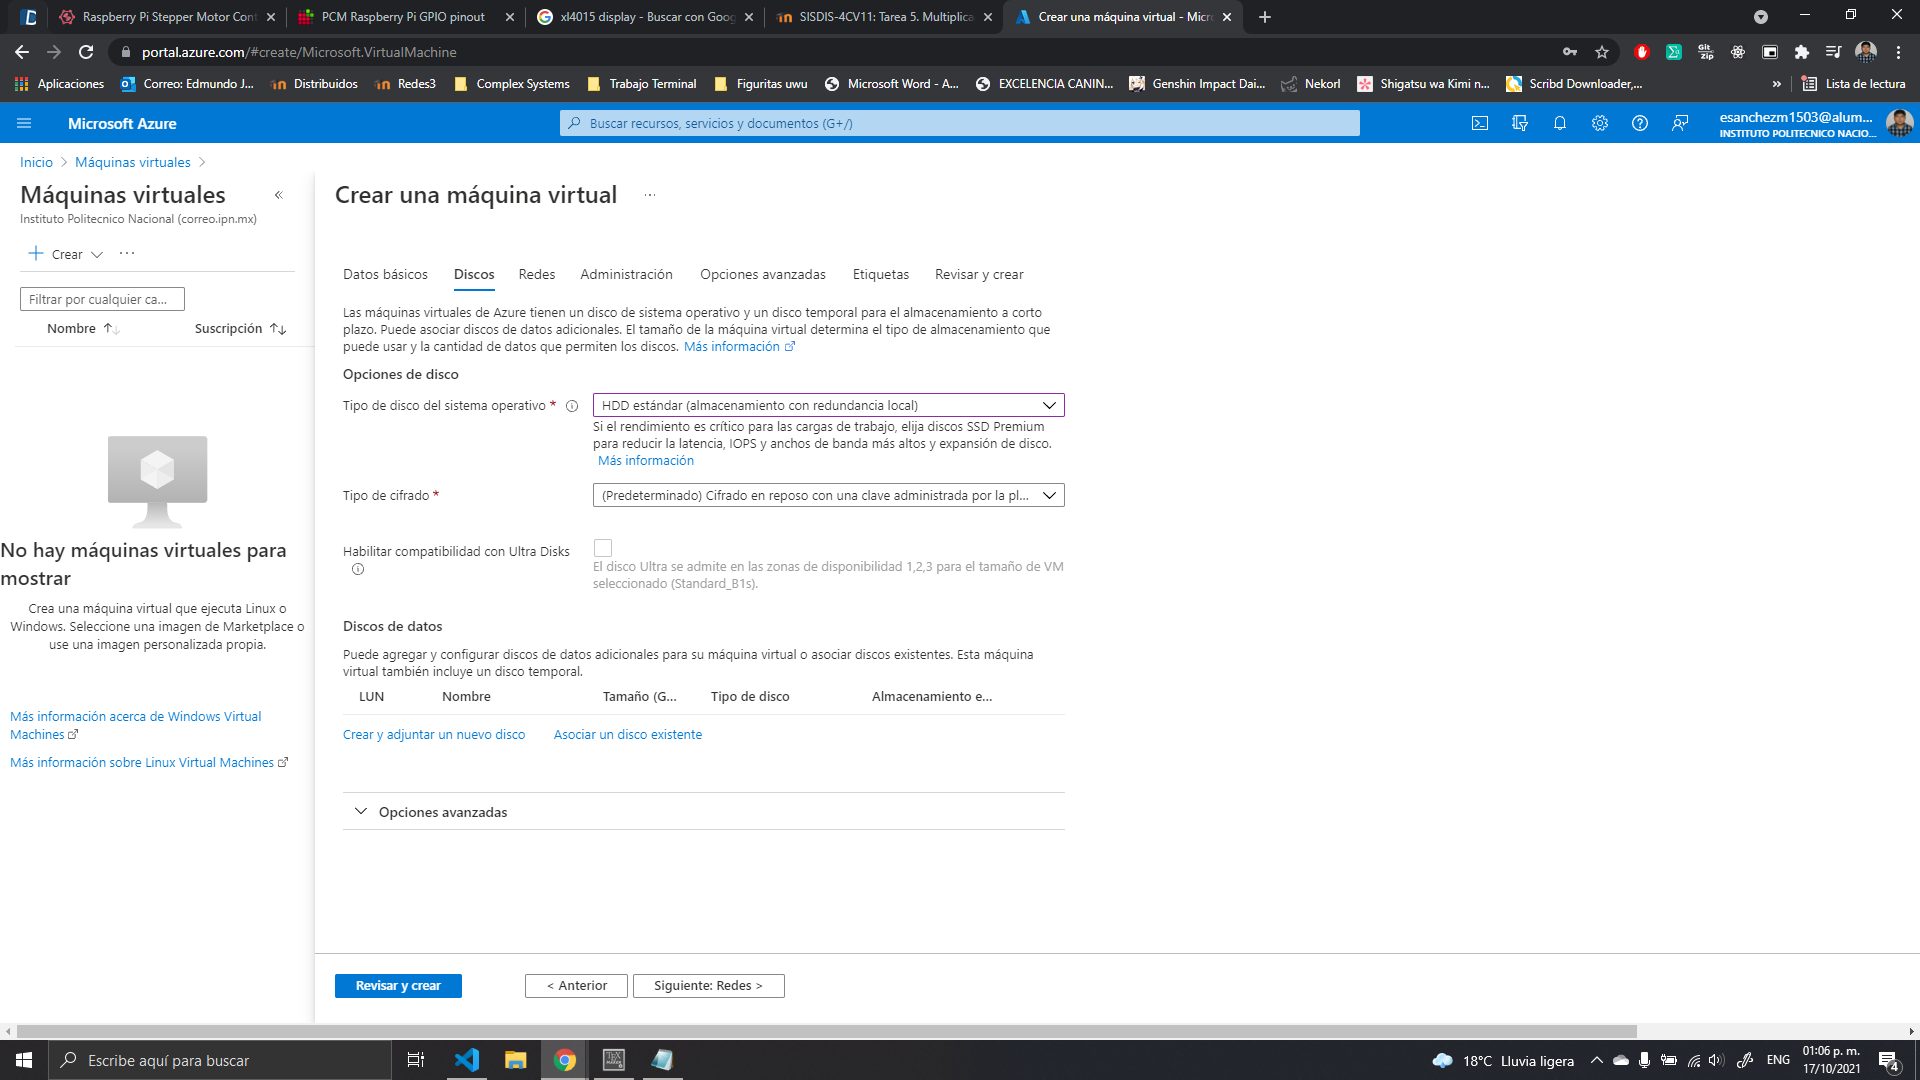
\includegraphics[scale=0.34]{resources/datosdisco.png}
			\caption{Configuración del tipo de disco para el nodo 0. }\label{fig:picture}
		\end{figure}
		\begin{figure}[H]
			\centering
			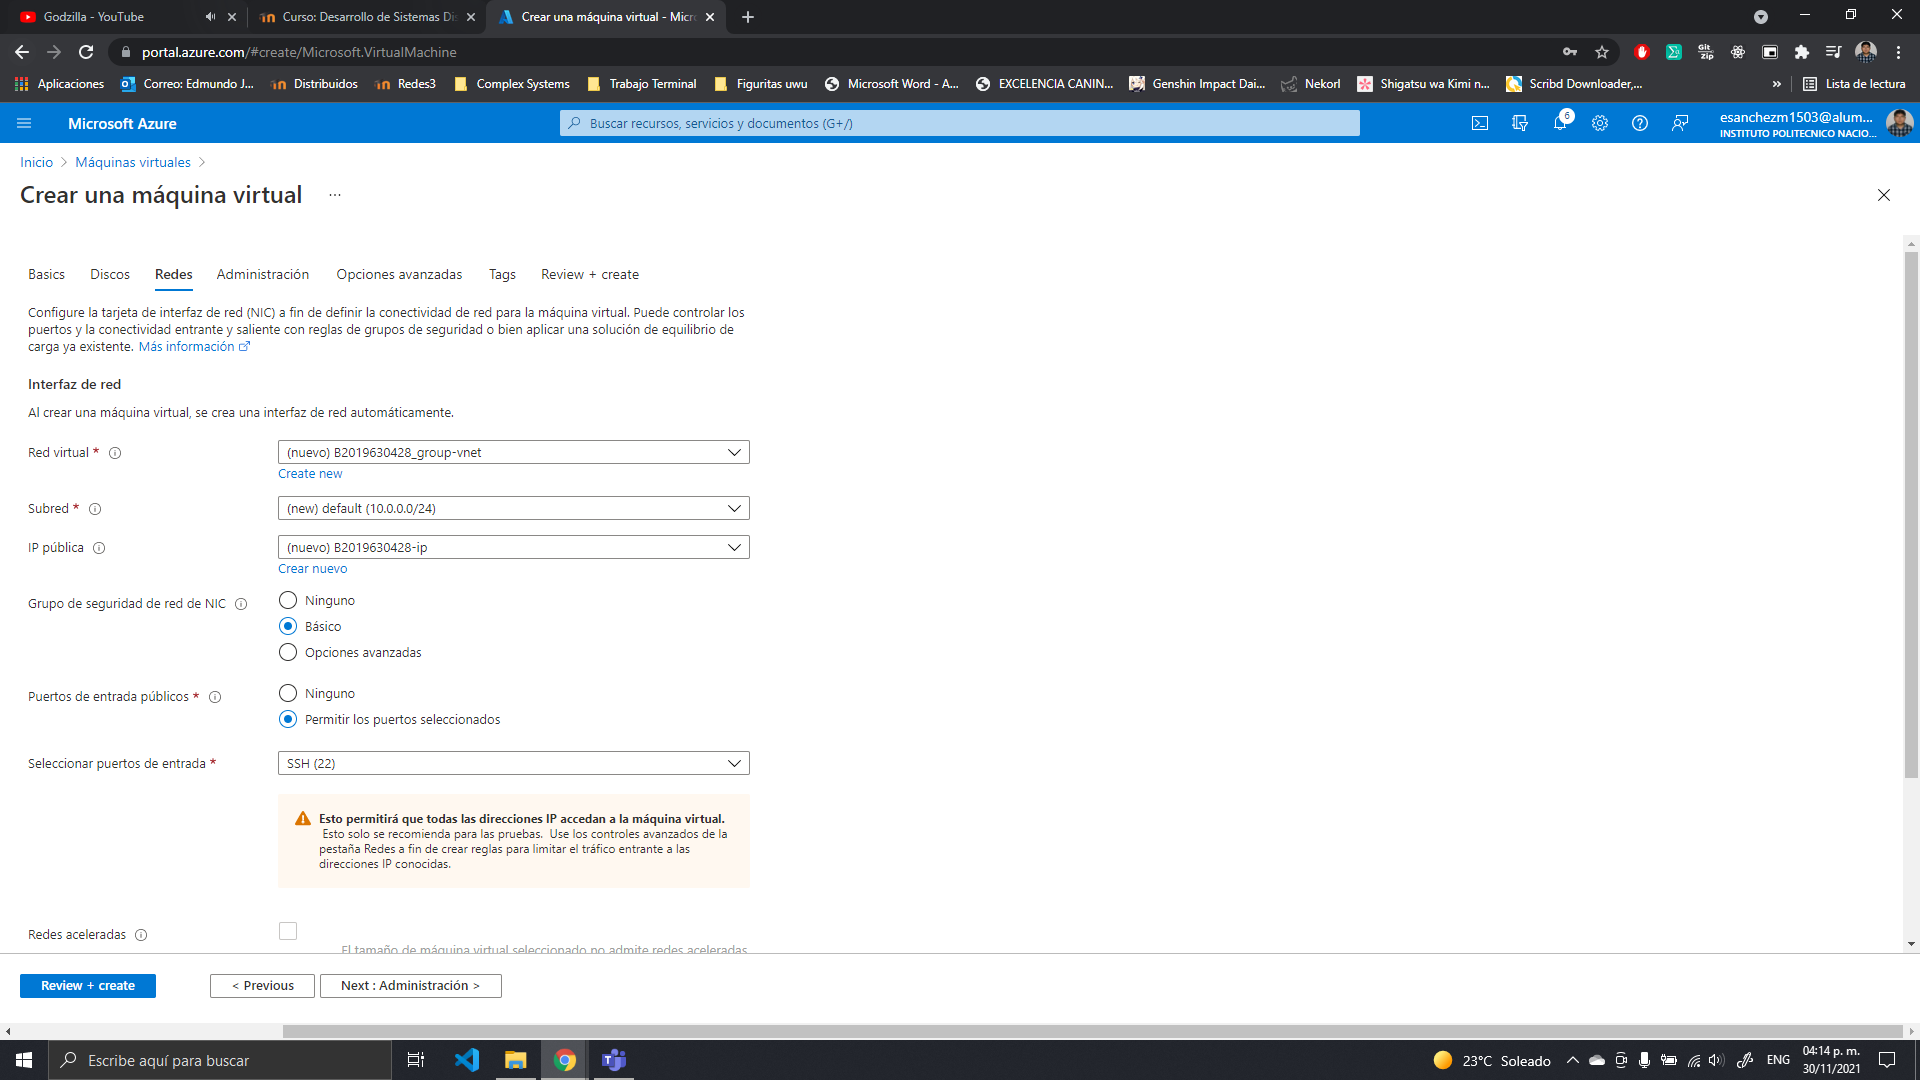
\includegraphics[scale=0.34]{resources/datosredes.png}
			\caption{Información sobre la redes para el nodo 0. }\label{fig:picture}
		\end{figure}
		\begin{figure}[H]
			\centering
			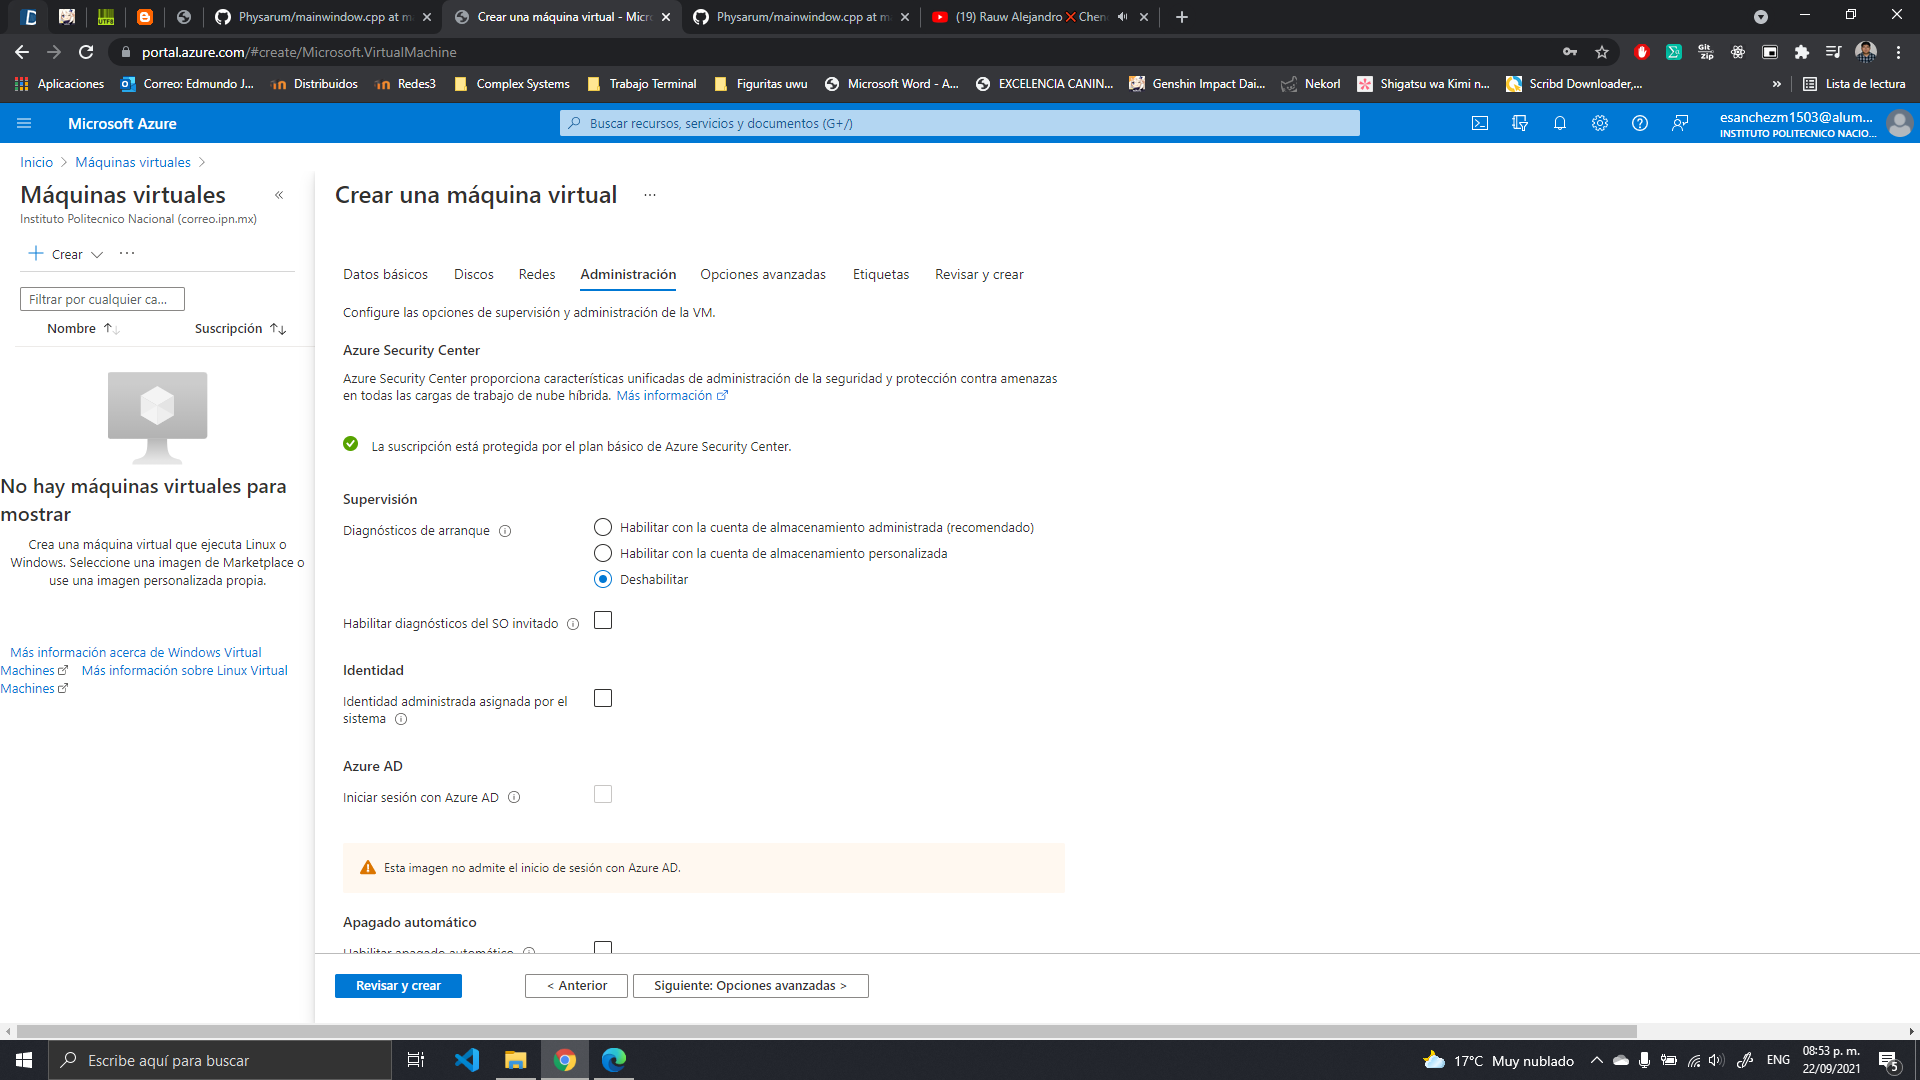
\includegraphics[scale=0.34]{resources/datosadministracion.png}
			\caption{Configuración de la administración para el nodo 0. }\label{fig:picture}
		\end{figure}
		\begin{figure}[H]
			\centering
			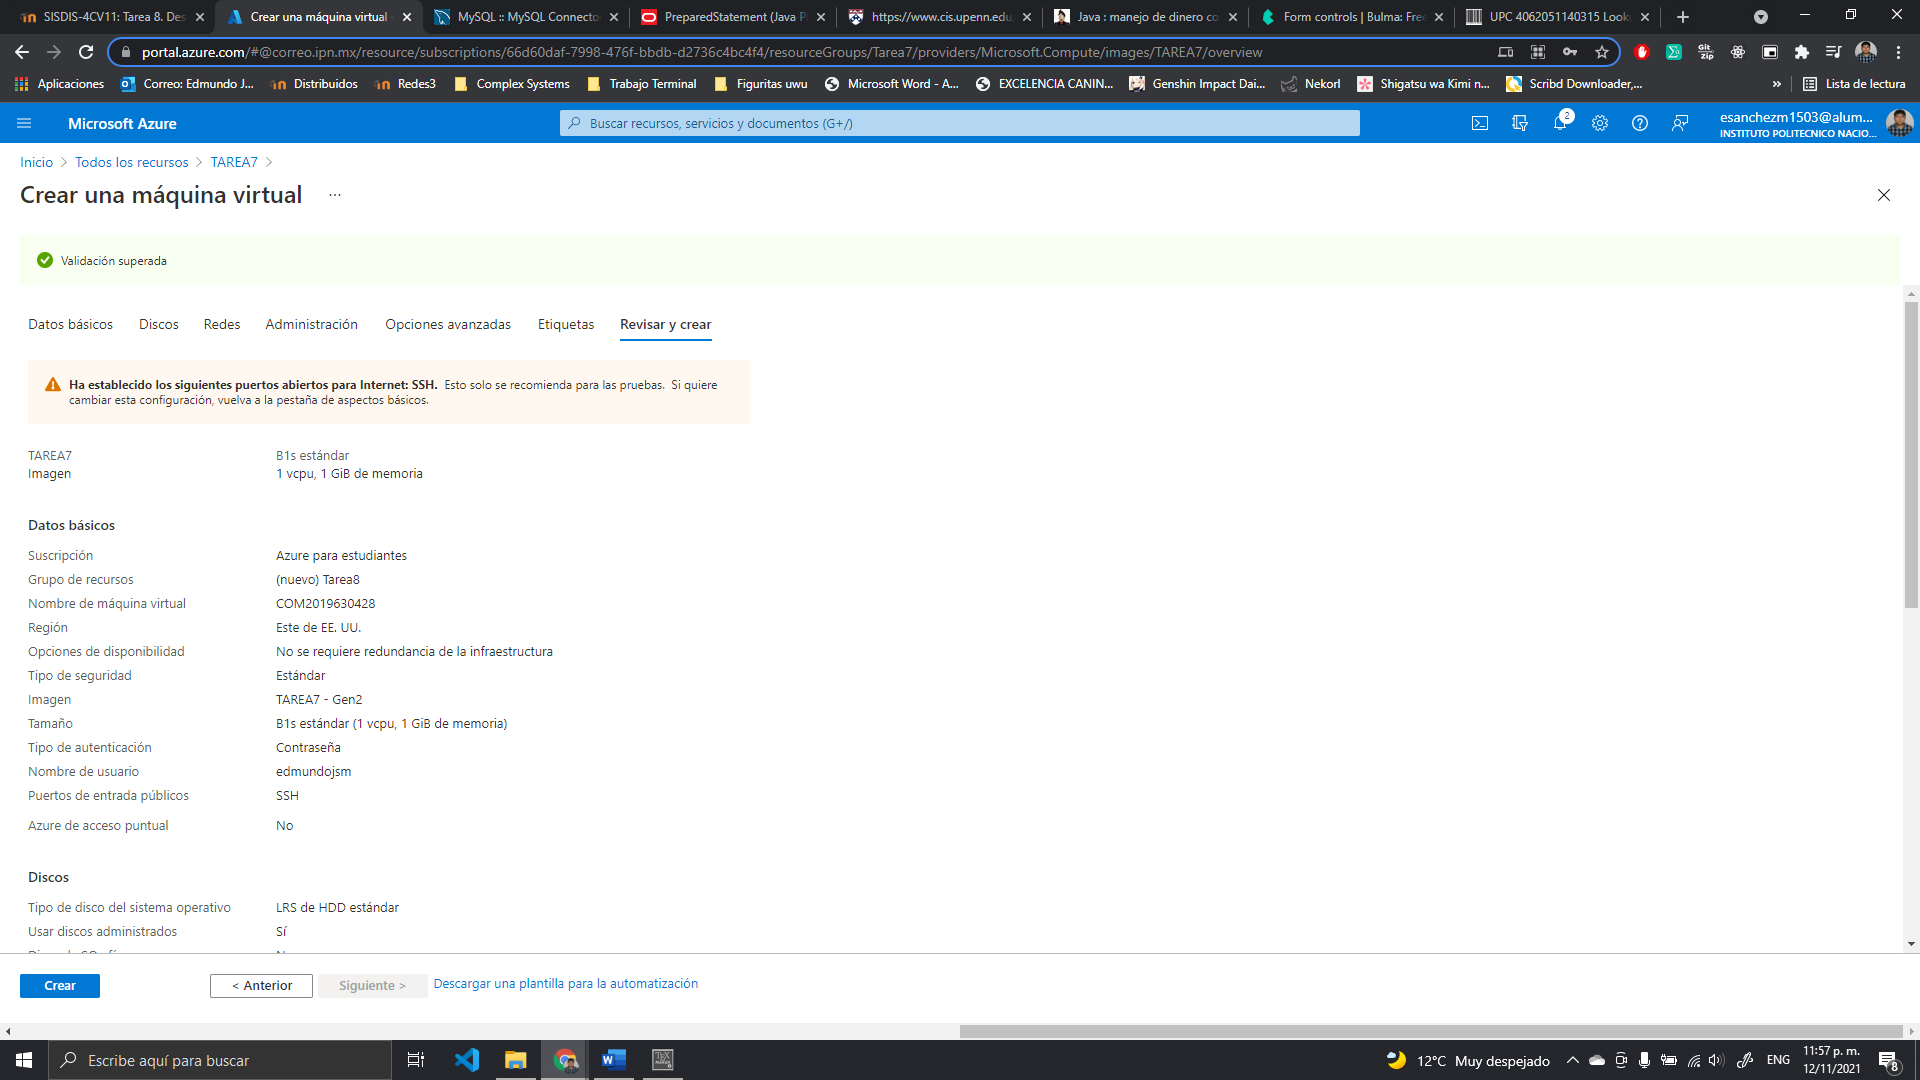
\includegraphics[scale=0.34]{resources/revisarycrear.png}
			\caption{Creación de la maquina virtual para el nodo 0. }\label{fig:picture}
		\end{figure}
		\begin{figure}[H]
			\centering
			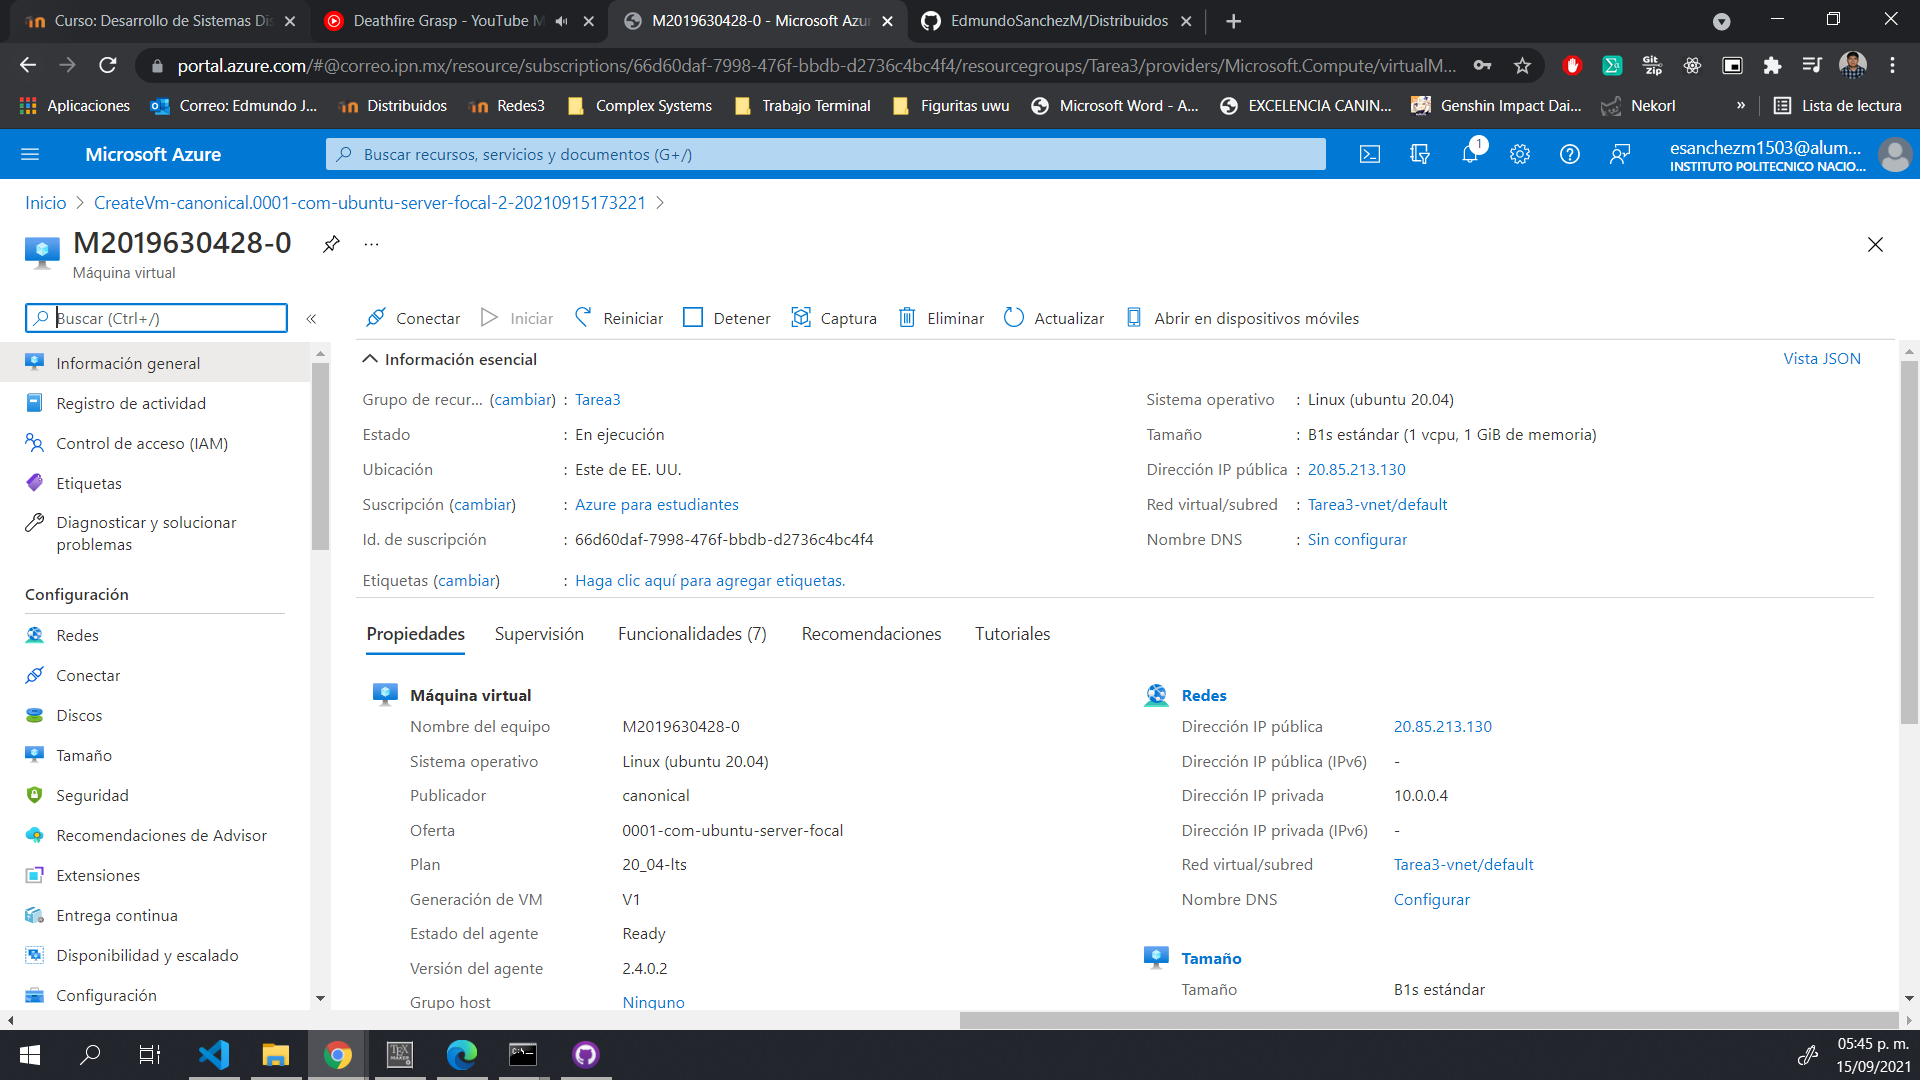
\includegraphics[scale=0.34]{resources/Panelcontrol.png}
			\caption{Panel de control de la maquina virtual para el nodo 0. }\label{fig:picture}
		\end{figure}
Las imágenes de la 1 a la 6 se tuvieron que repetir tres veces mas, esto debido al tipo de topologia a implementar, mencionar que en mi caso al momento de querer crear una quinta maquina virtual con las características dadas en la tarea no se me dejo, ya que tengo un limite de 4 maquinas al usar standar\_ B1, por lo que tuve que crear una maquina virtual con otras características, intente aumentar el limite que tengo pero no me fue posible ya que me solicitan crear un token con el soporte técnico, sin embargo, al usar una maquina con otras características aparentemente no me genero un gran costo como pensaba que seria.\par
El cliente RMI ejecutará en una máquina virtual con Ubuntu en Azure (nodo 0). El servidor RMI ejecutará en tres máquinas virtuales (nodo 1, nodo 2 y nodo 3) con Ubuntu en Azure. El programa rmiregistry ejecutará en cada nodo donde ejecute el servidor RMI. El nodo 1 calculará los productos C1, C2 y C3, el nodo 2 calculará los productos C4, C5 y C6, y el nodo 3 calculará los productos C7, C8 y C9, antes de probar nuestro programa necesitamos hacer uso de las IP privadas de los nodos 1, 2 y 3, esto implica crear 3 lookup para cada nodo, esto para poder distribuir el calculo de las matrices ya que el nodo 1 calculará los productos C1, C2 y C3, el nodo 2 calculará los productos C4, C5 y C6, y el nodo 3 calculará los productos C7, C8 y C9.\par
Una vez creadas las maquinas virtuales se procedió a hacer lo que se muestra en las figuras de 7 y 8 por las 4 maquinas que tenemos, usamos como ejemplo el nodo 0
		\begin{figure}[H]
			\centering
			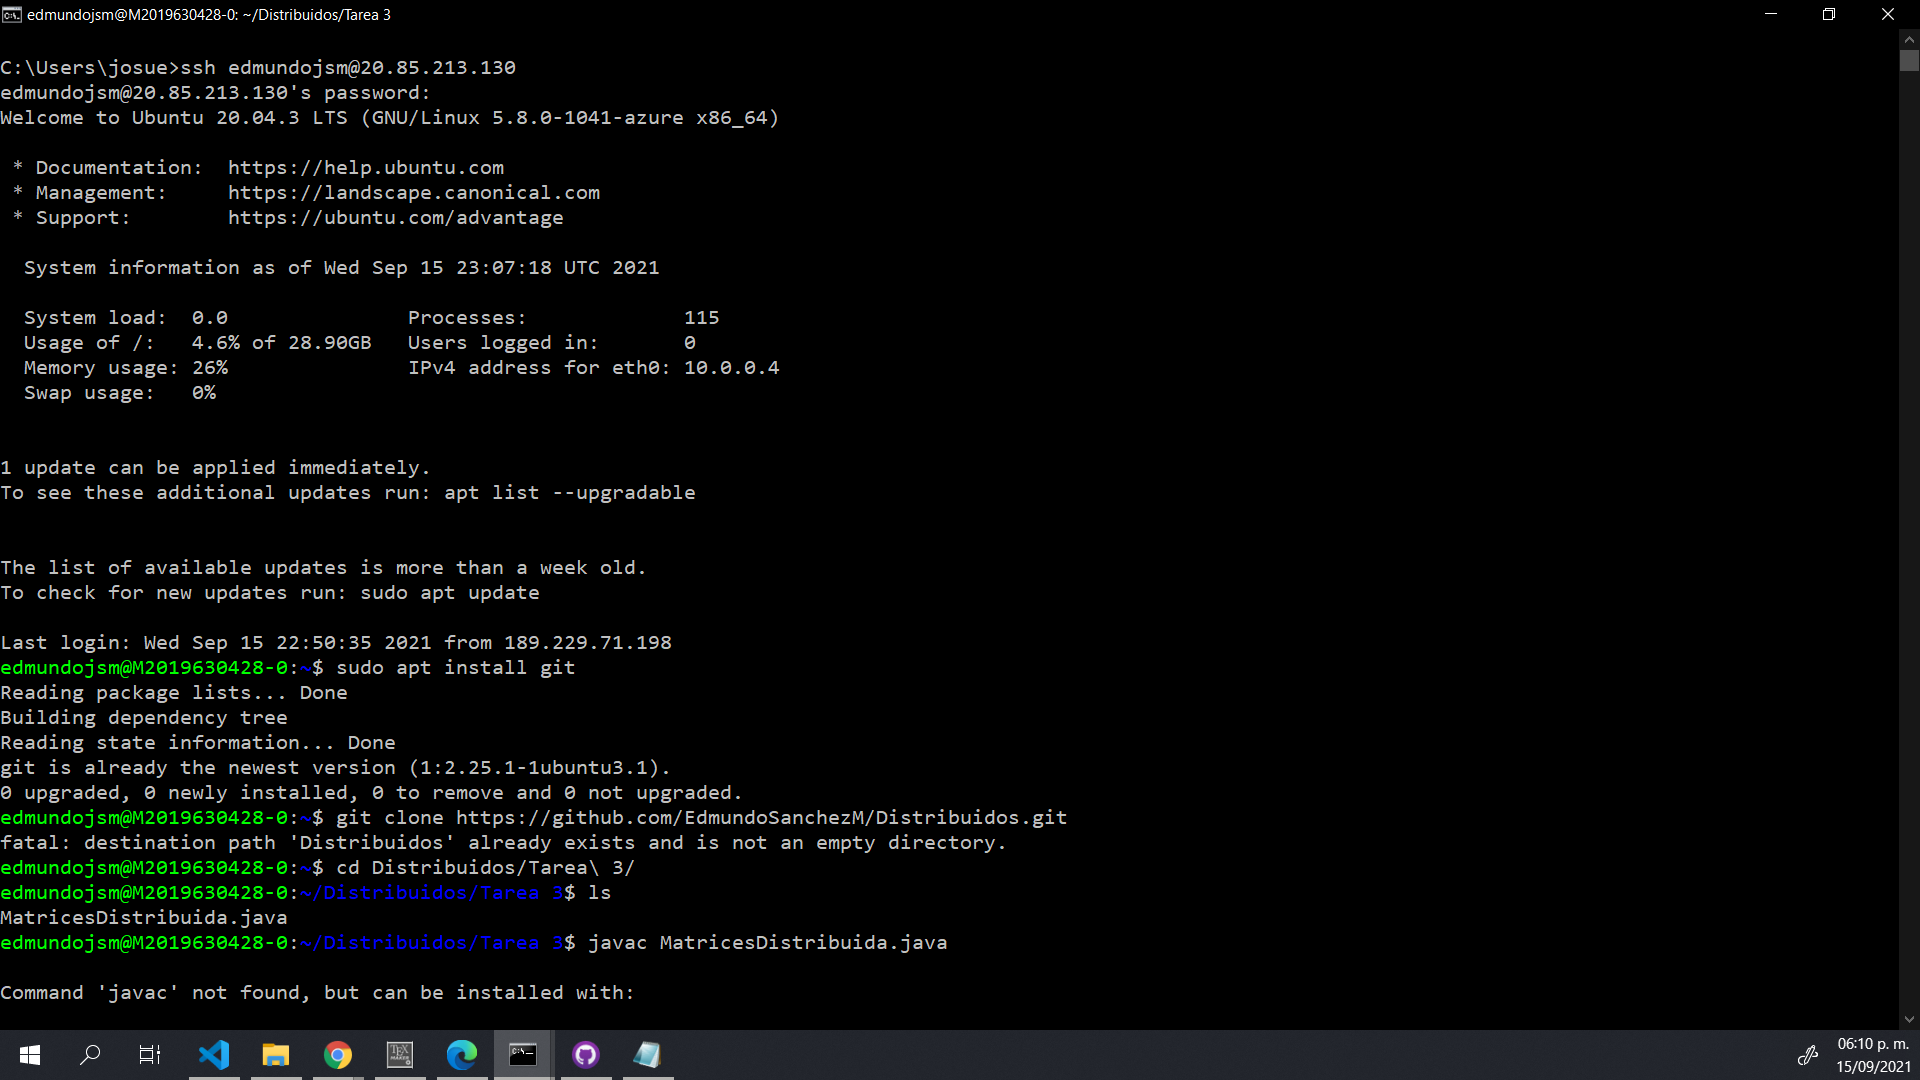
\includegraphics[scale=0.34]{resources/Nodo0ssh.png}
			\caption{Conexión vía ssh a la maquina virtual que hará como nodo 0. }\label{fig:picture}
		\end{figure}
		\begin{figure}[H]
			\centering
			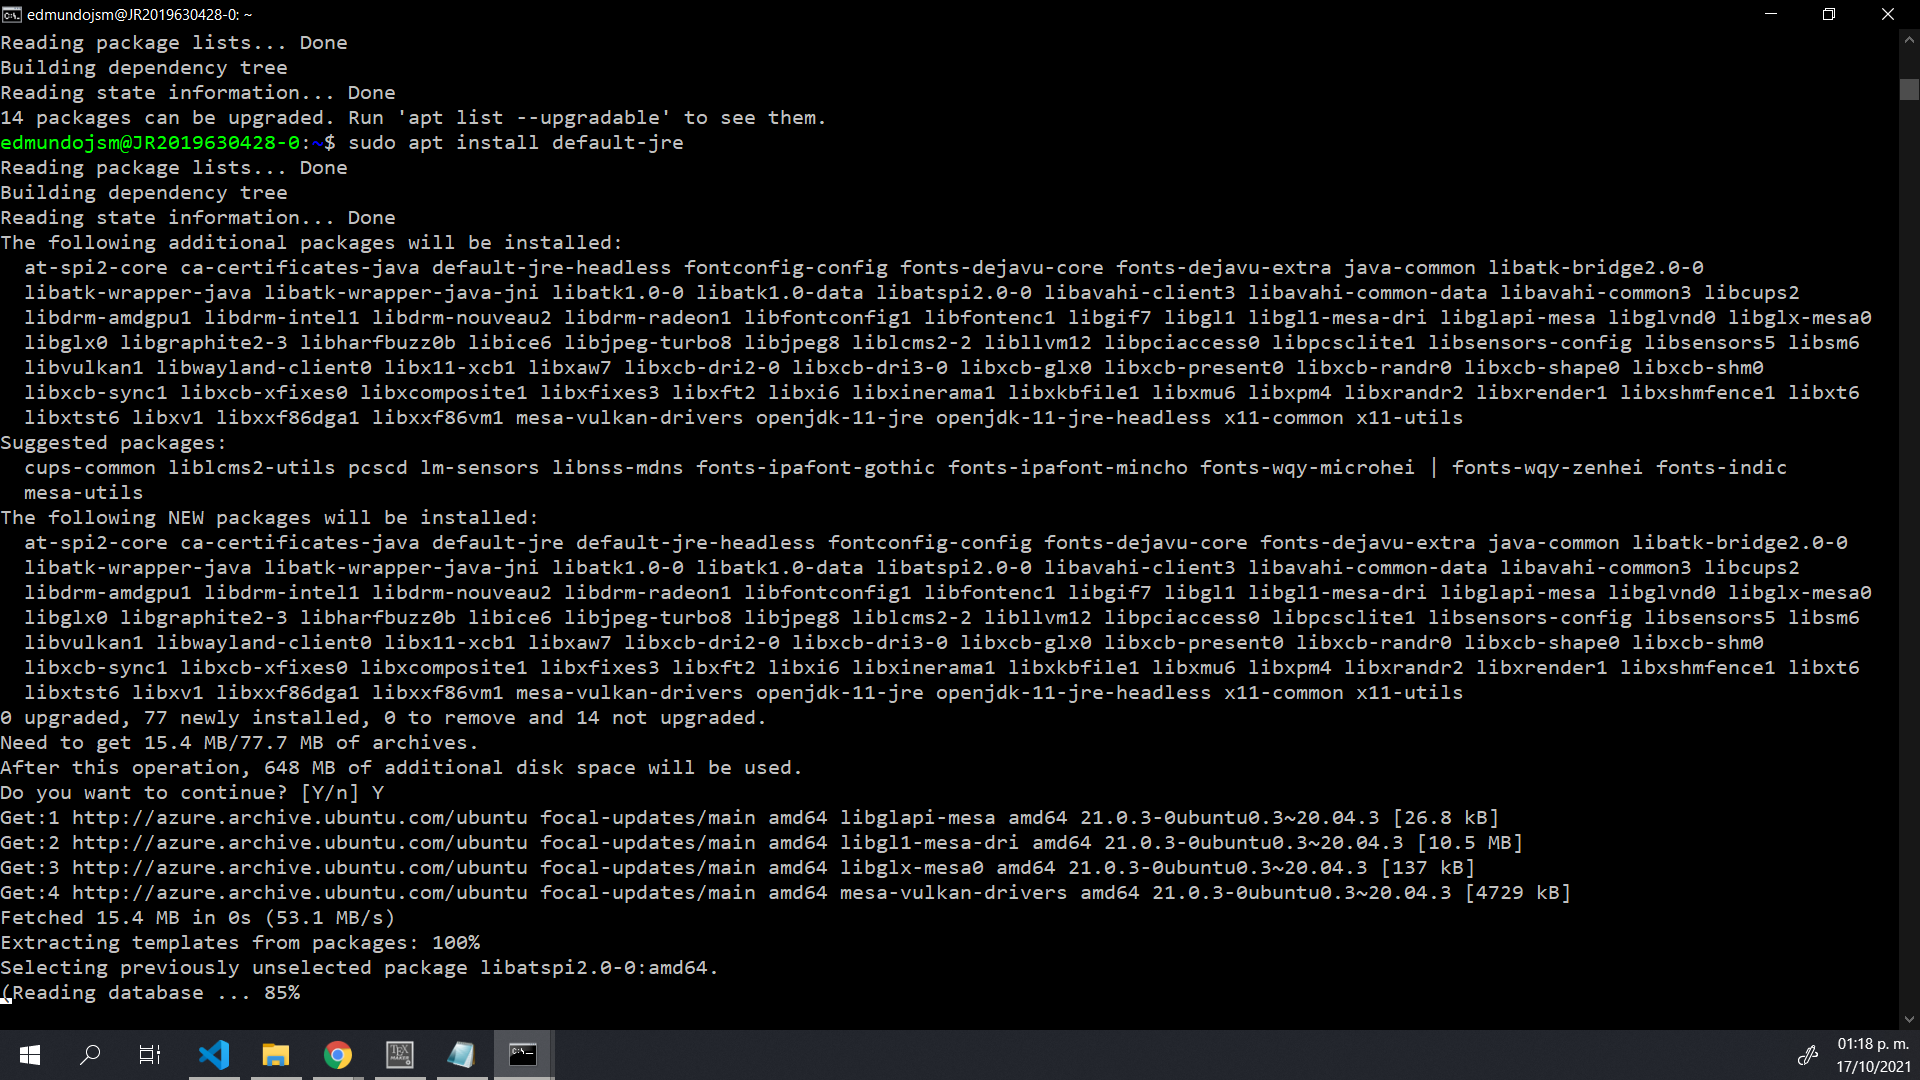
\includegraphics[scale=0.34]{resources/instalarjava.png}
			\caption{Instalación del jdk en el nodo 0. }\label{fig:picture}
		\end{figure}
		Una vez configurado cada maquina virtual se procedió a enviar los archivos por medio de WinSCP el cual solo es necesario arrastrar los archivos a usar a la maquina virtual y eso es todo, una vez copiado los archivos correspondientes a cada nodo procedemos a la compilación del código.
		\subsection{Compilación del código}
		En la figura 9 podemos ver como la compilación del archivo ClienteRMI.java e InterfaceRMI.java en el nodo 0, ademas de que en la figura 10 podemos ver la compilación de los archivos  InterfaceRMI.java, ServidorRMI.java y ClaseRMI.java en el nodo 1 esta compilación se hace de manera exitosa y sin ningún error alguno, esto desde la terminal de Ubuntu de nuestras maquinas virtuales, recordar que lo que se hizo en el nodo 1 se repite en los nodos 2 y 3.
		\begin{figure}[H]
			\centering
			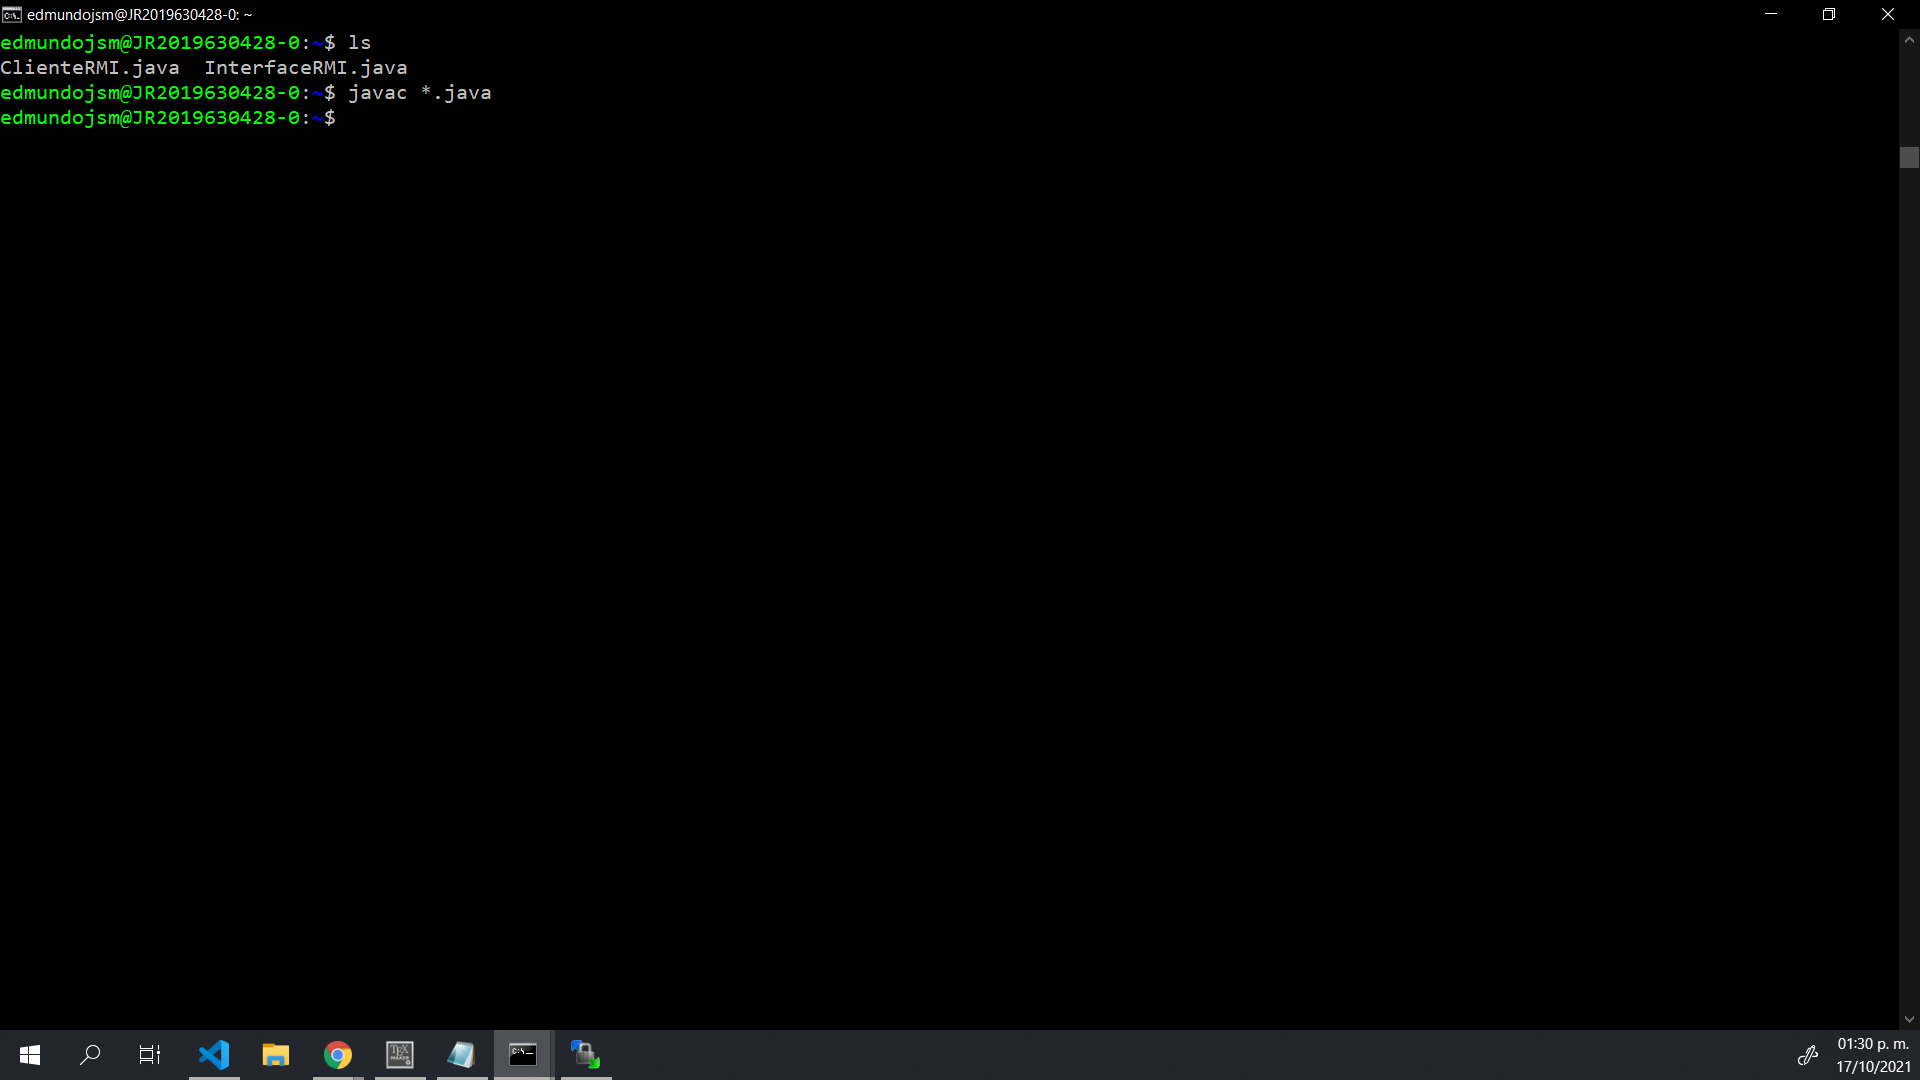
\includegraphics[scale=0.34]{resources/compilacionClienteInterface.png}
				\caption{Compilación del código ClienteRMI.java e InterfaceRMI.java en el nodo 0. }					\label{fig:picture}
		\end{figure}
		
		\begin{figure}[H]
			\centering
			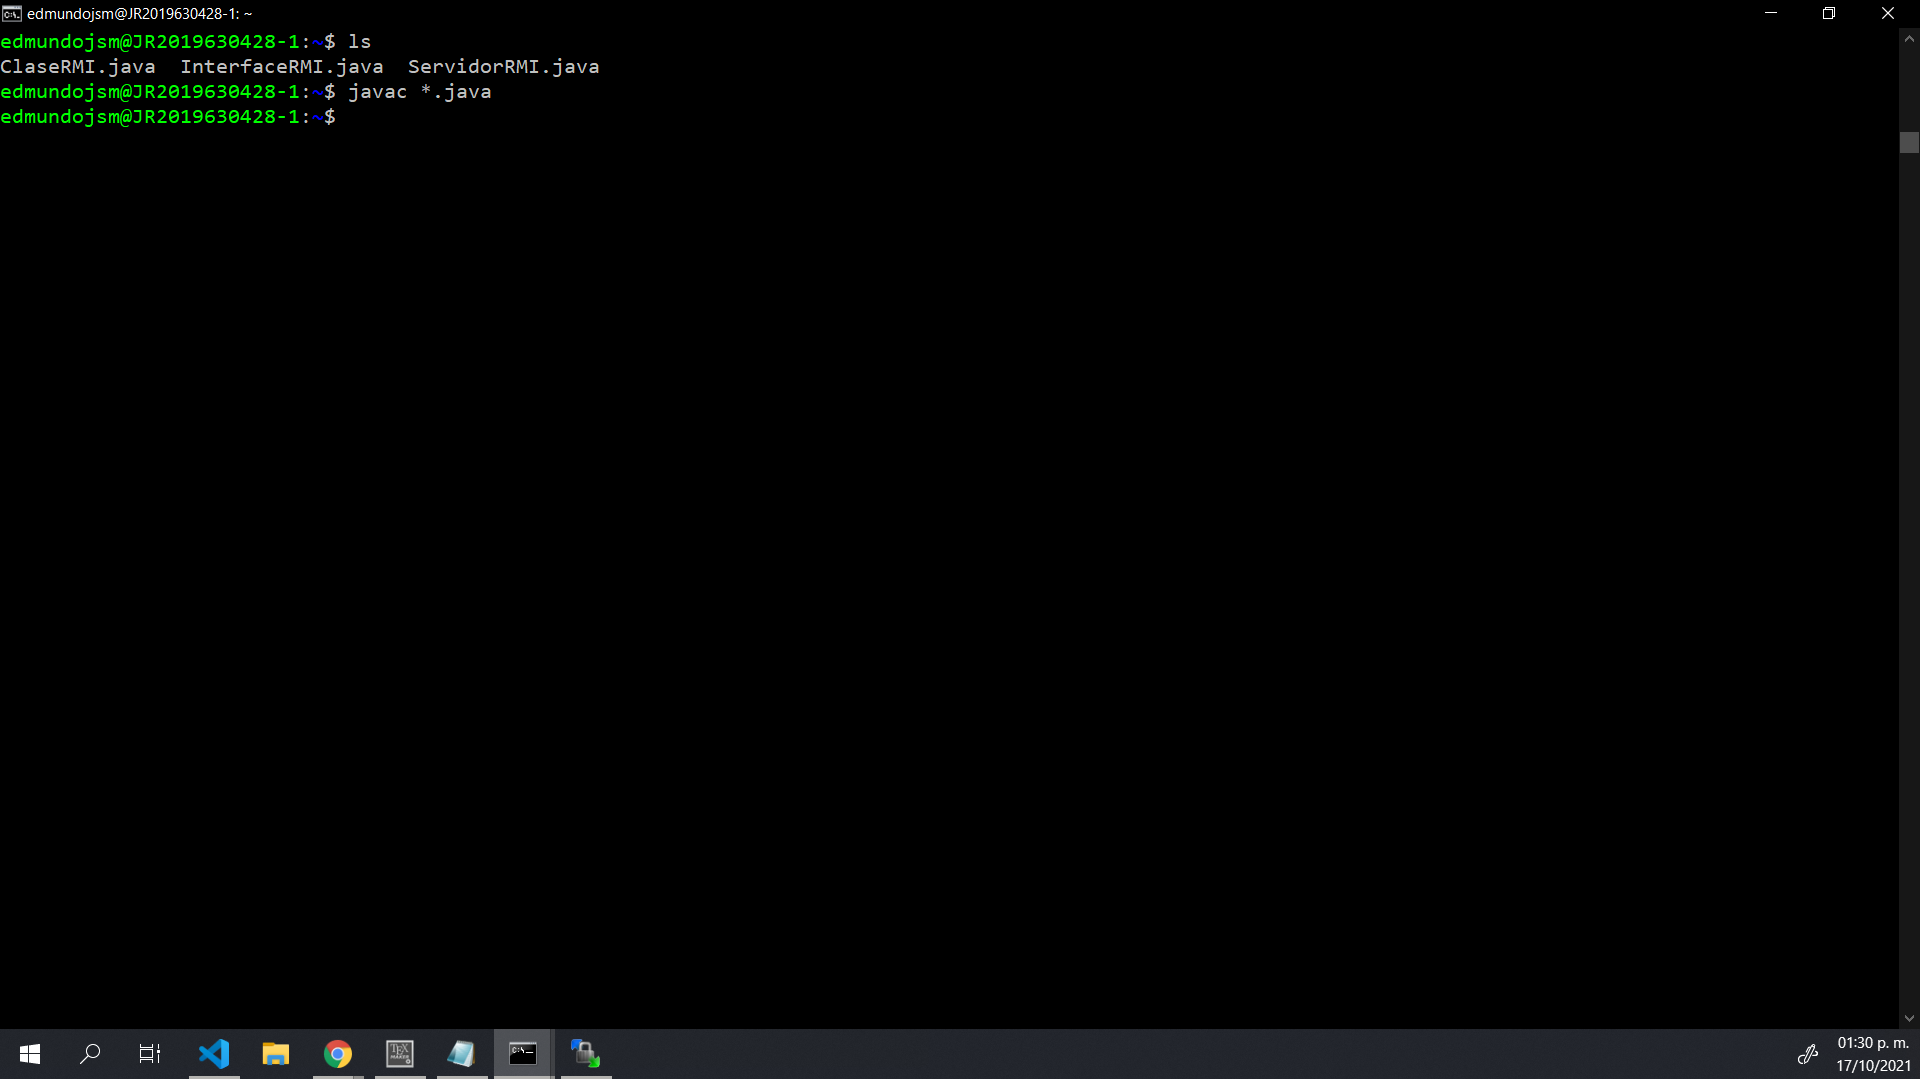
\includegraphics[scale=0.34]{resources/compilacionlodemasxd.png}
				\caption{Compilación de los archivos  InterfaceRMI.java, ServidorRMI.java y ClaseRMI.java en el nodo 1.}					\label{fig:picture}
		\end{figure}
		\subsection{Ejecución del programa}
		Antes de ir con las pruebas necesarias para la entrega de esta tarea en la imagen 11 podemos ver la ejecución de los servidores RMI y rmiregistry en las terminales de los nodos 1, 2 y 3.
		\begin{figure}[H]
			\centering
			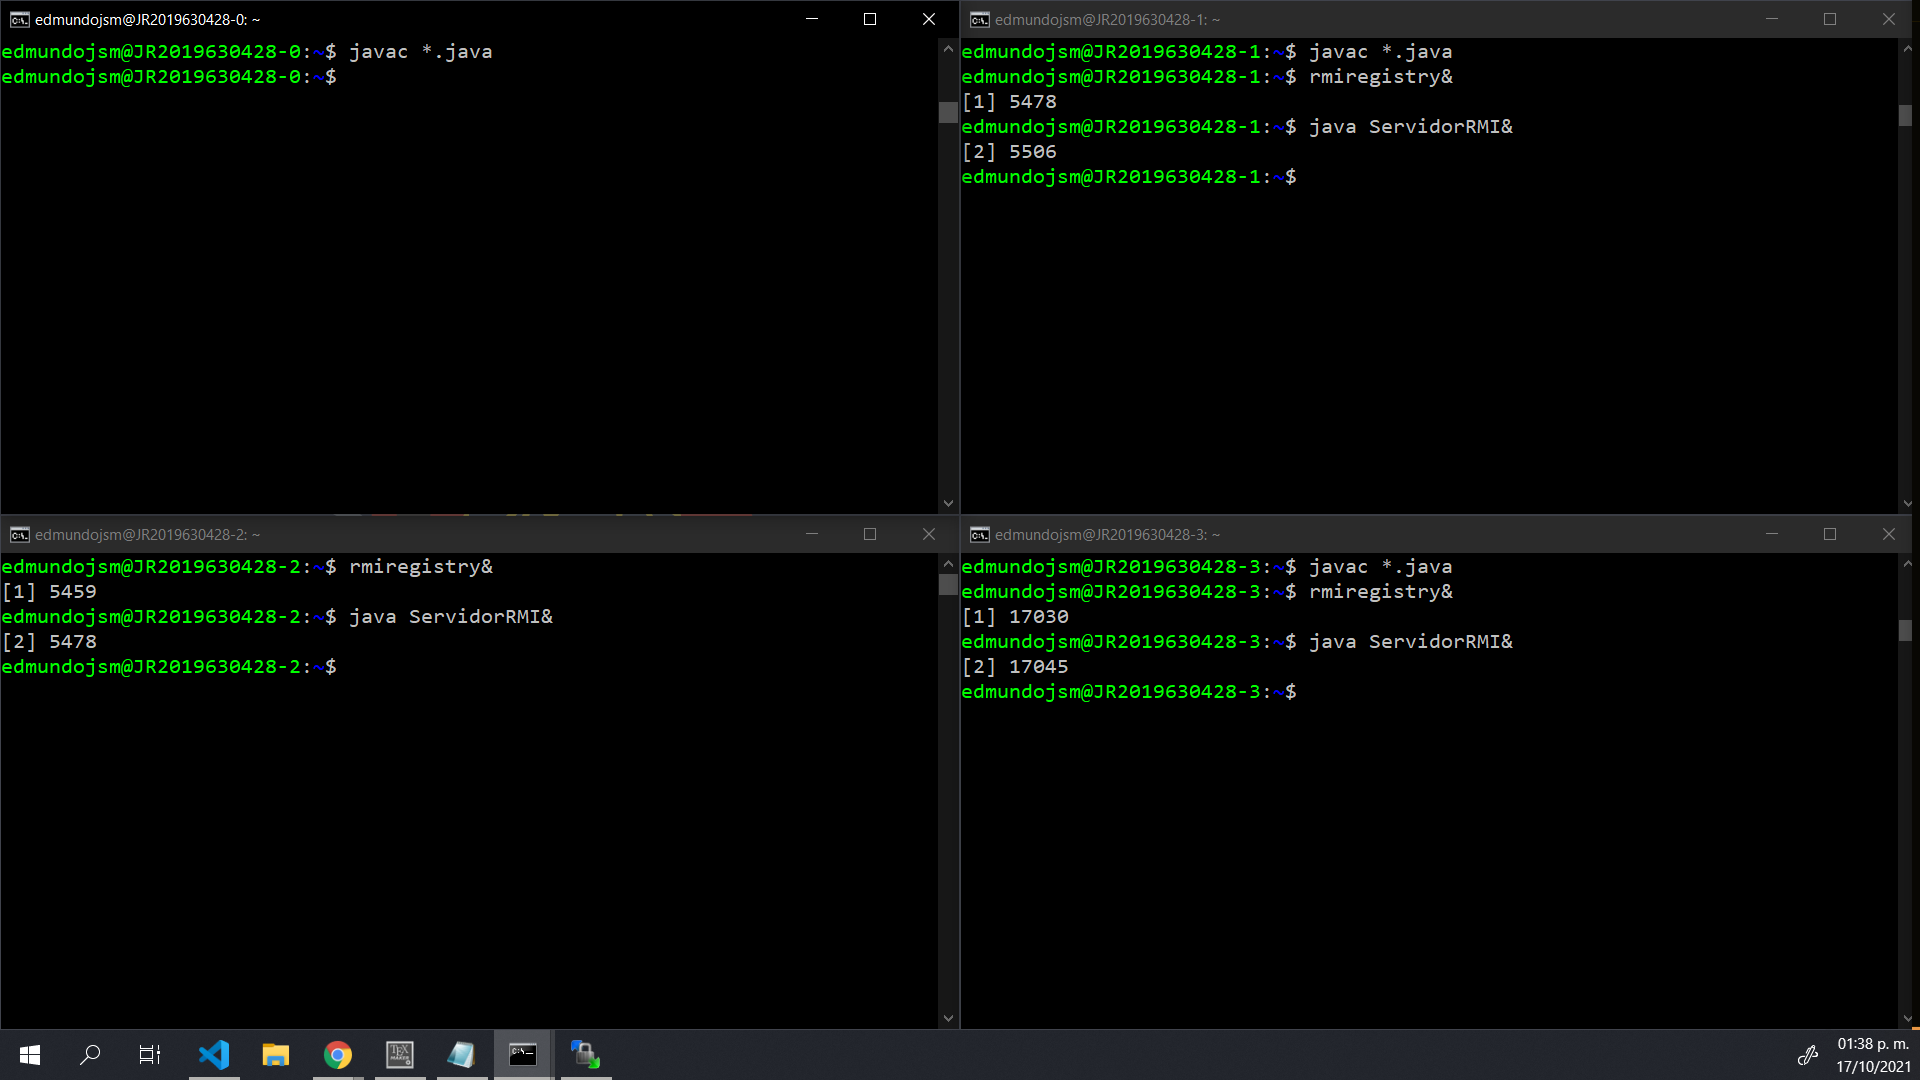
\includegraphics[scale=0.34]{resources/servidores.png}
			\caption{Ejecución del programa ServidorRMI en los nodos 1, 2 y 3. }\label{fig:picture}
		\end{figure}
		\subsubsection{N=9}
		Una vez compilado nuestro programa en cada maquina virtual se procede a la ejecución del cliente RMI y como vemos en la figura 12 podemos ver como se nos imprime el valor de la matriz A, la matriz B antes de ser transpuesta, la matriz C y el valor de checksum de la matriz c.
		\begin{figure}[H]
			\centering
			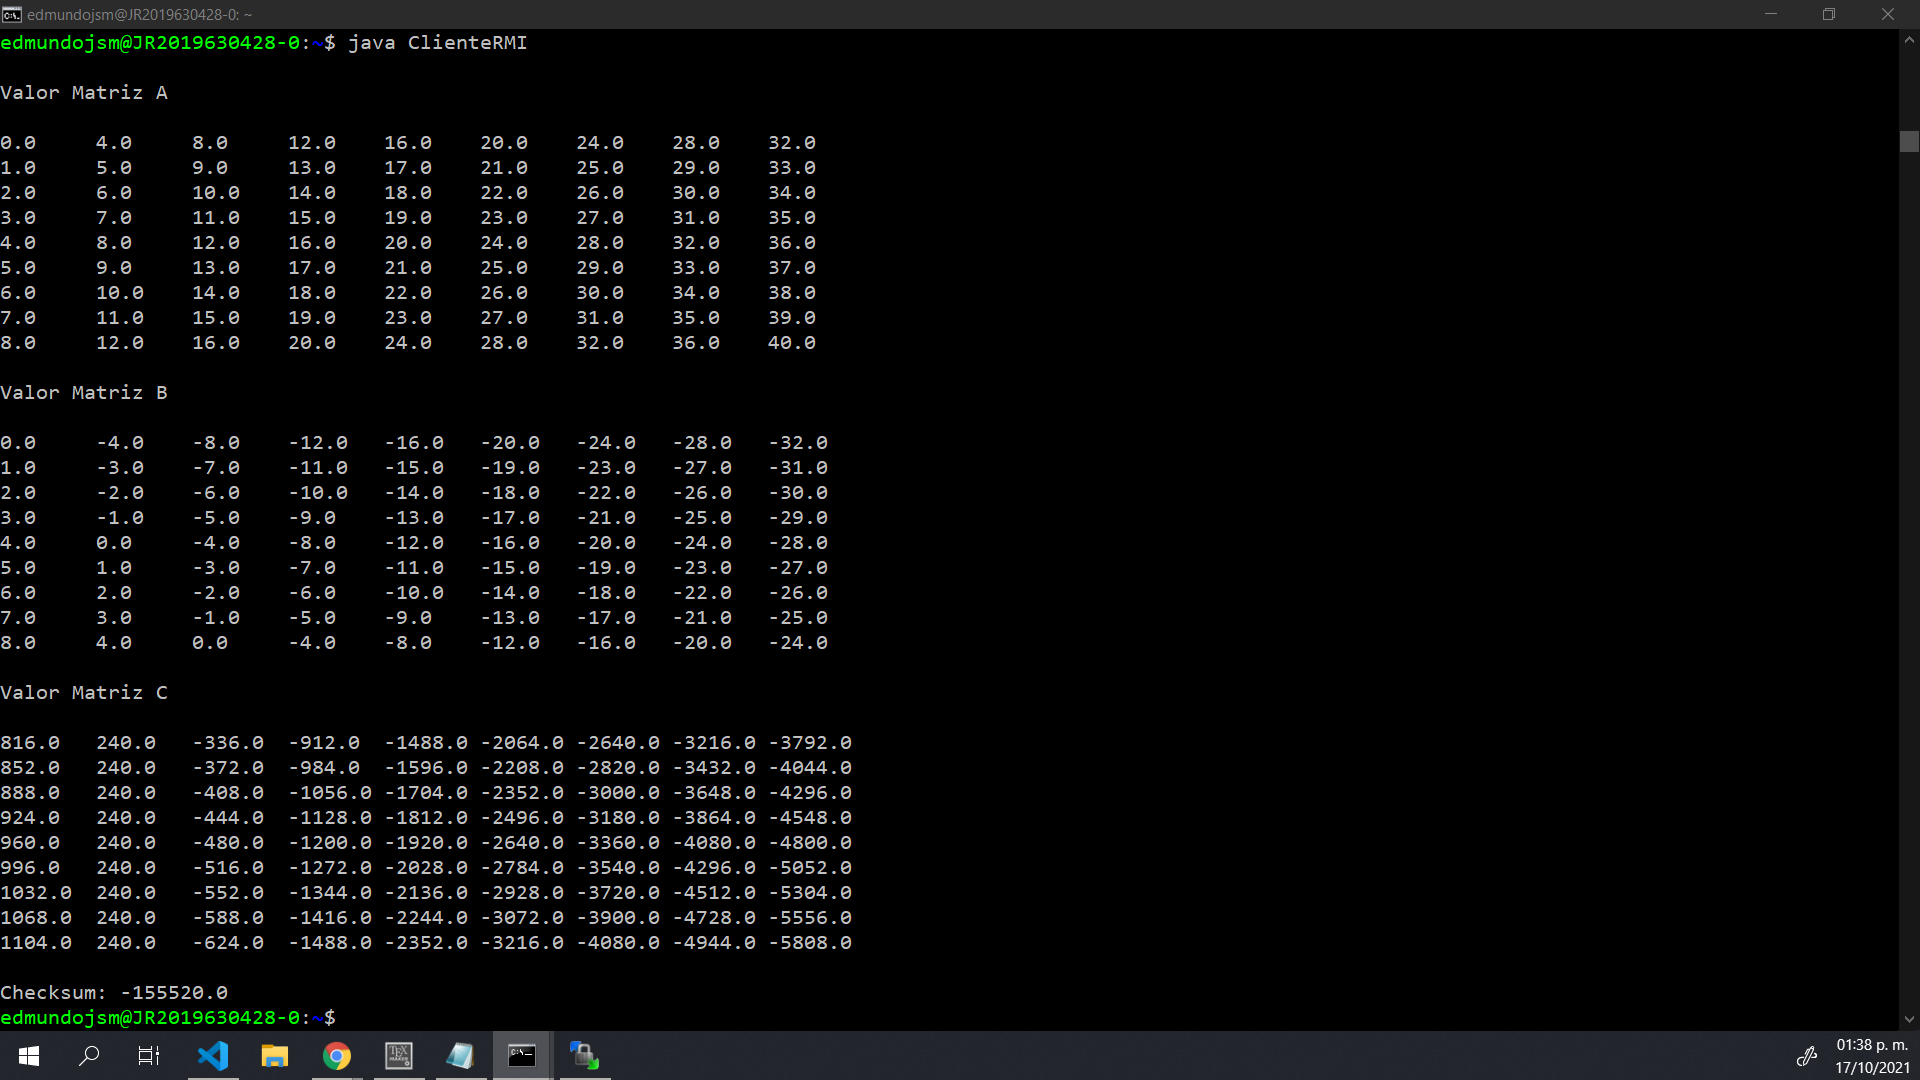
\includegraphics[scale=0.34]{resources/hacksuwul.png}
			\caption{Valor de checksum para N=9 y valores de las matrices A, B y c. }\label{fig:picture}
		\end{figure}
		Ahora veamos el siguiente caso con N=3000.
		\subsubsection{N=3000}
		Para este caso se tuvo que modificar el programa asignando 3000 esto por medio del uso del comando nano ClienteRMI.java en el nodo 0 para poder cambiar el valor de N como vemos en la figura 13
		\begin{figure}[H]
			\centering
			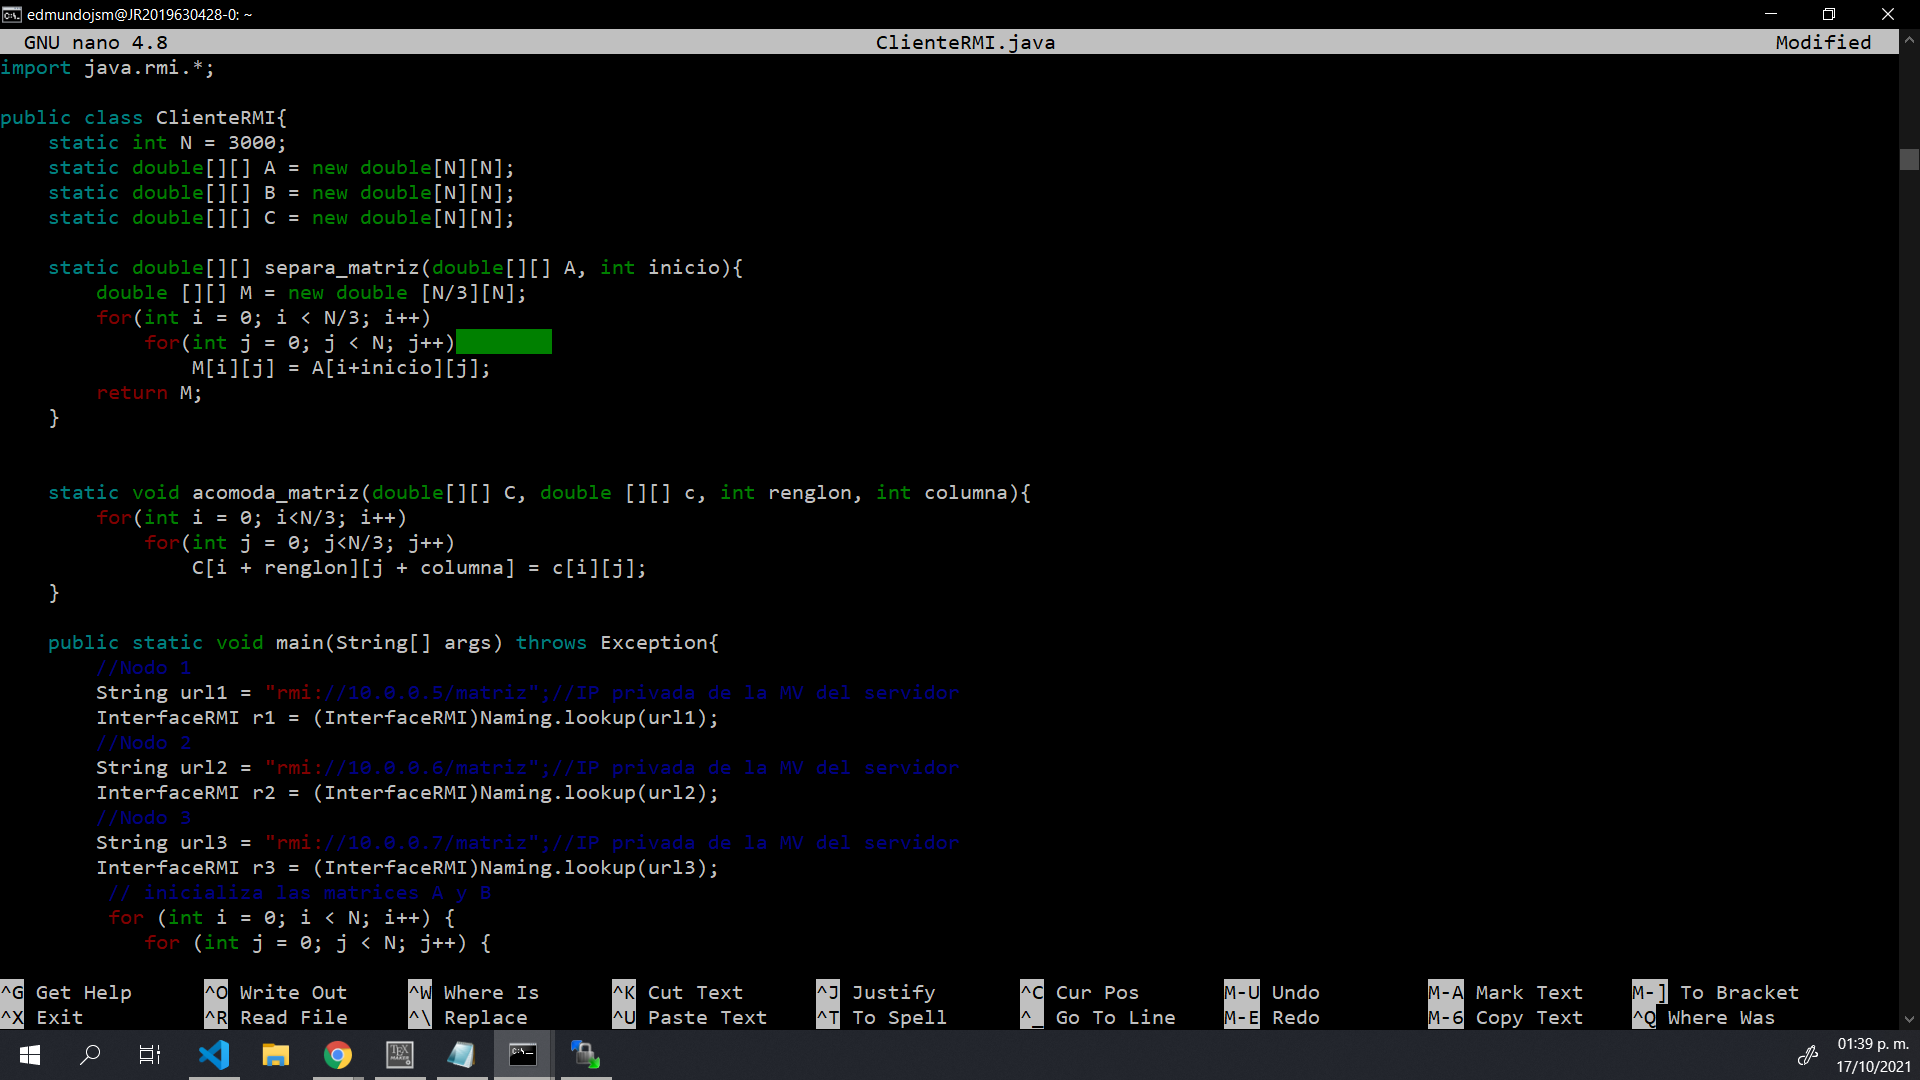
\includegraphics[scale=0.34]{resources/config3000.png}
			\caption{Modificación del valor de N de 9 a 3000. }\label{fig:picture}
		\end{figure}
		Antes de ver el resultado de valor del checksum calculado sucedió algo interesante y es que como vemos en la figura 14 nos salio un error el cual nos indica que no tenemos suficiente cantidad de memoria para poder separar la matriz, para poder solucionar esto, la única solución era aumentar la memoria de la maquina virtual como podemos ver en la figura 15.
		\begin{figure}[H]
			\centering
			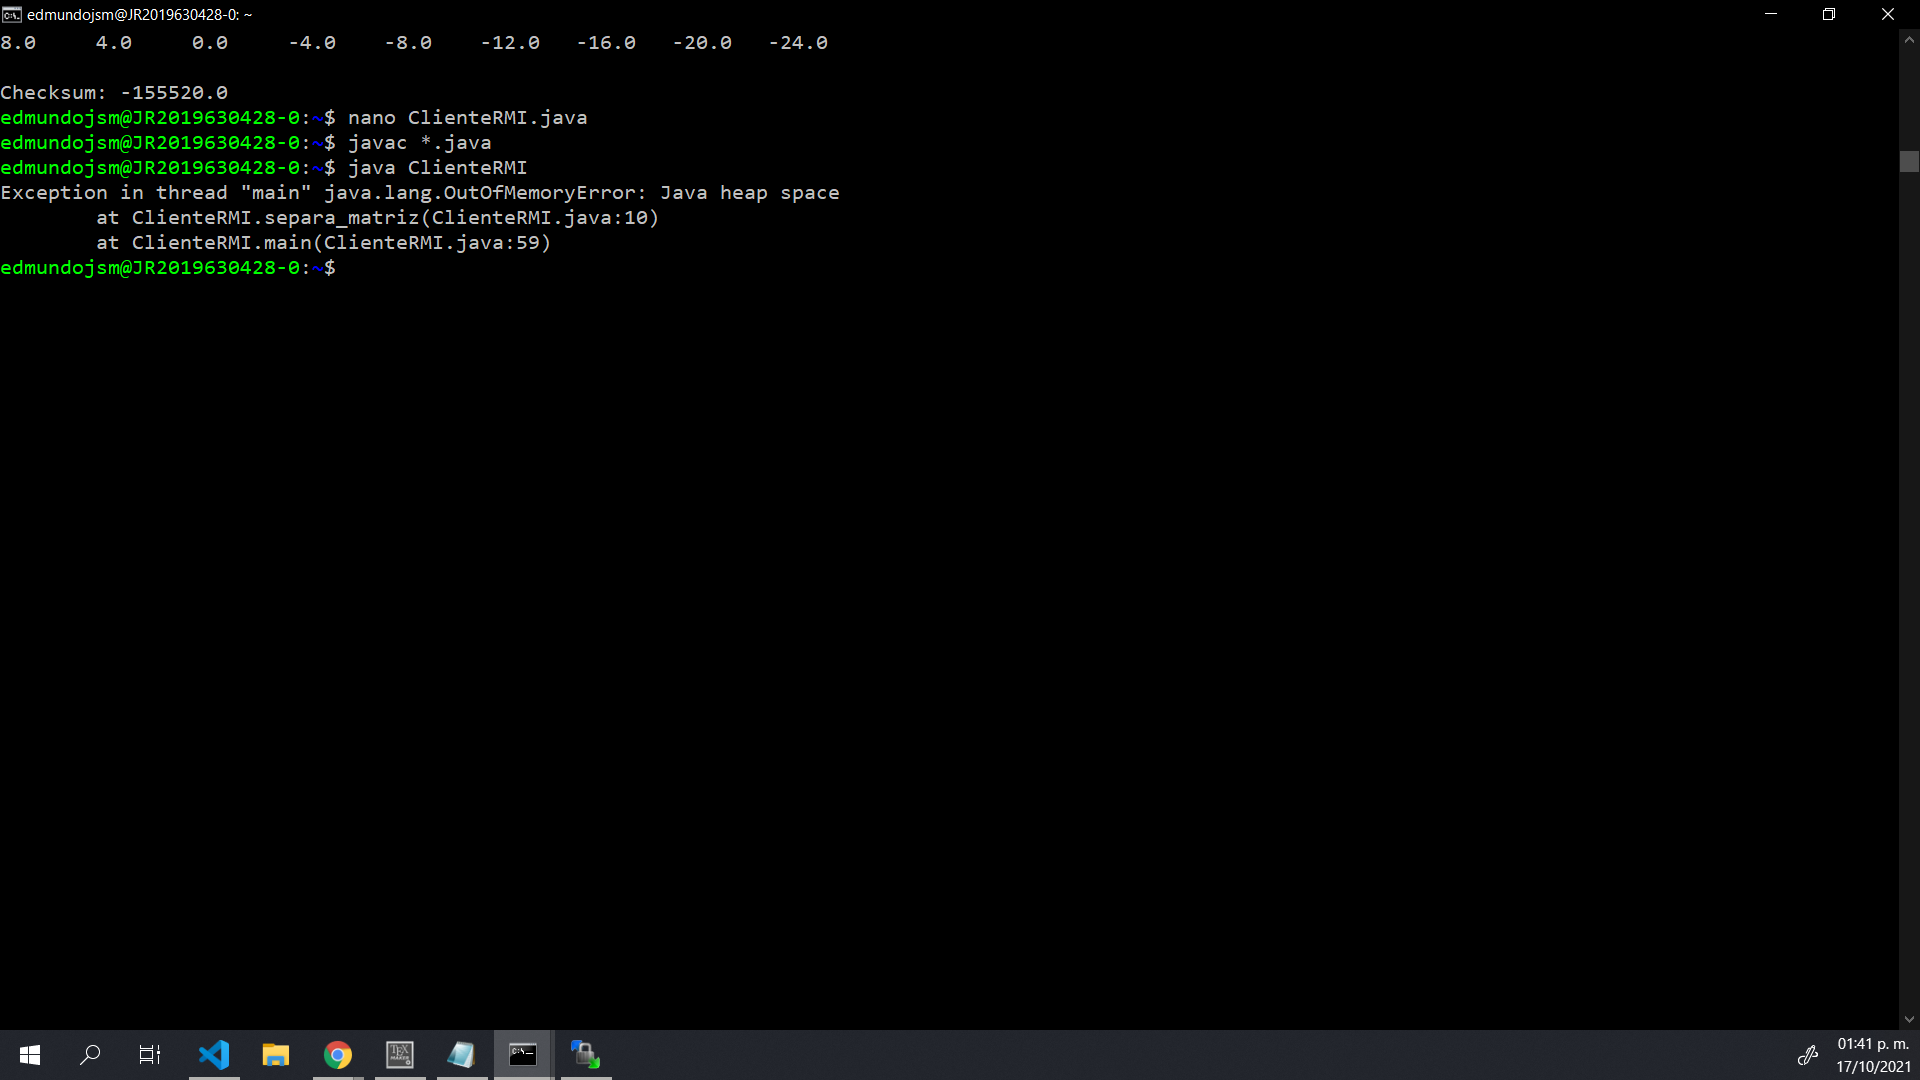
\includegraphics[scale=0.34]{resources/error.png}
			\caption{Error al ejecutar el programa.}\label{fig:picture}
		\end{figure}
		\begin{figure}[H]
			\centering
			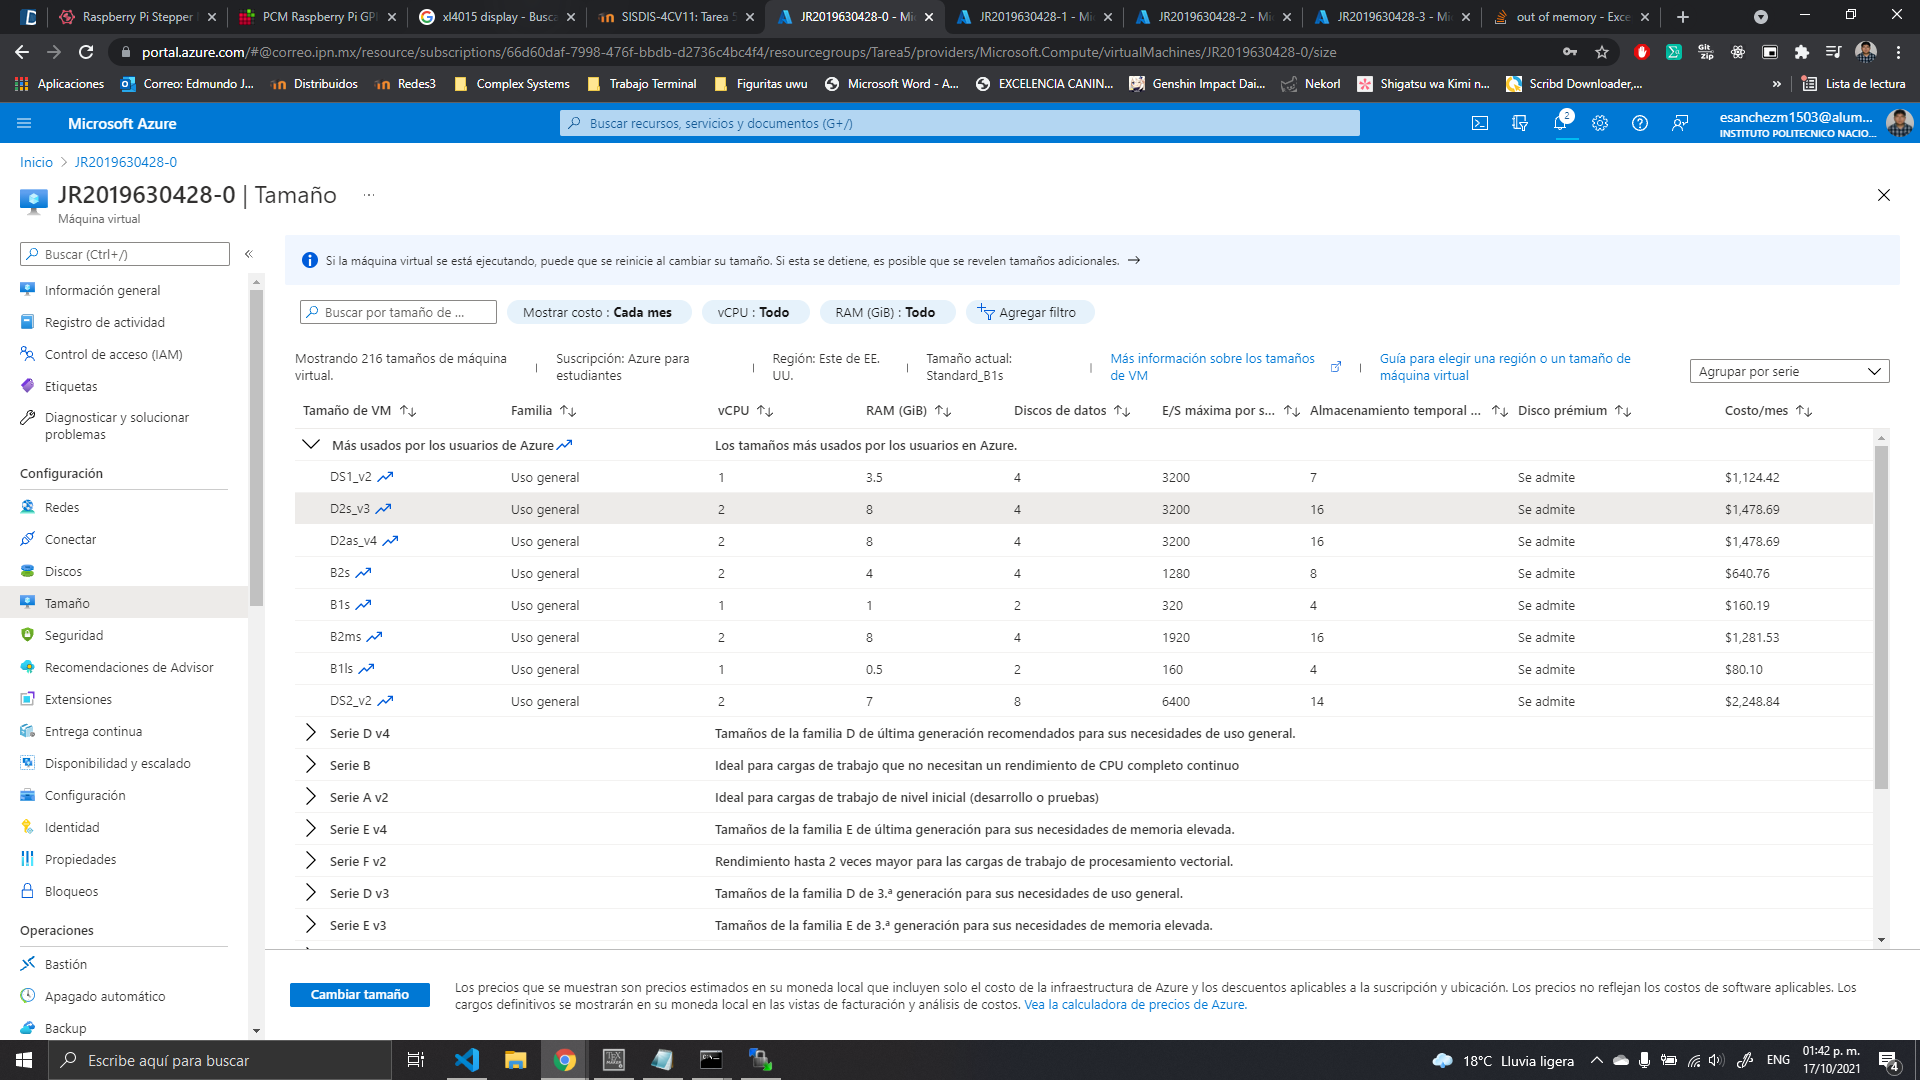
\includegraphics[scale=0.34]{resources/cambiandotama.png}
			\caption{Cambiando el tamaño de la maquina virtual del nodo 0.}\label{fig:picture}
		\end{figure}
		Si vemos la figura 6 en donde podemos ver la cantidad de memoria RAM que poseía el nodo 0 es de 1 RAM, al hacer la actualización a 8 de RAM ya no tenemos ese problema, sin embargo puede que nos estemos preguntando, entonces porque en los servidores no salio ningún error y es que al dividir las matrices en 3 nos facilita el manejo del tamaño de 3000 elementos y esto provoca que las maquinas restantes no sufran de este error, sin embargo, es evidente que la ejecución sera lenta.\par
		\begin{figure}[H]
			\centering
			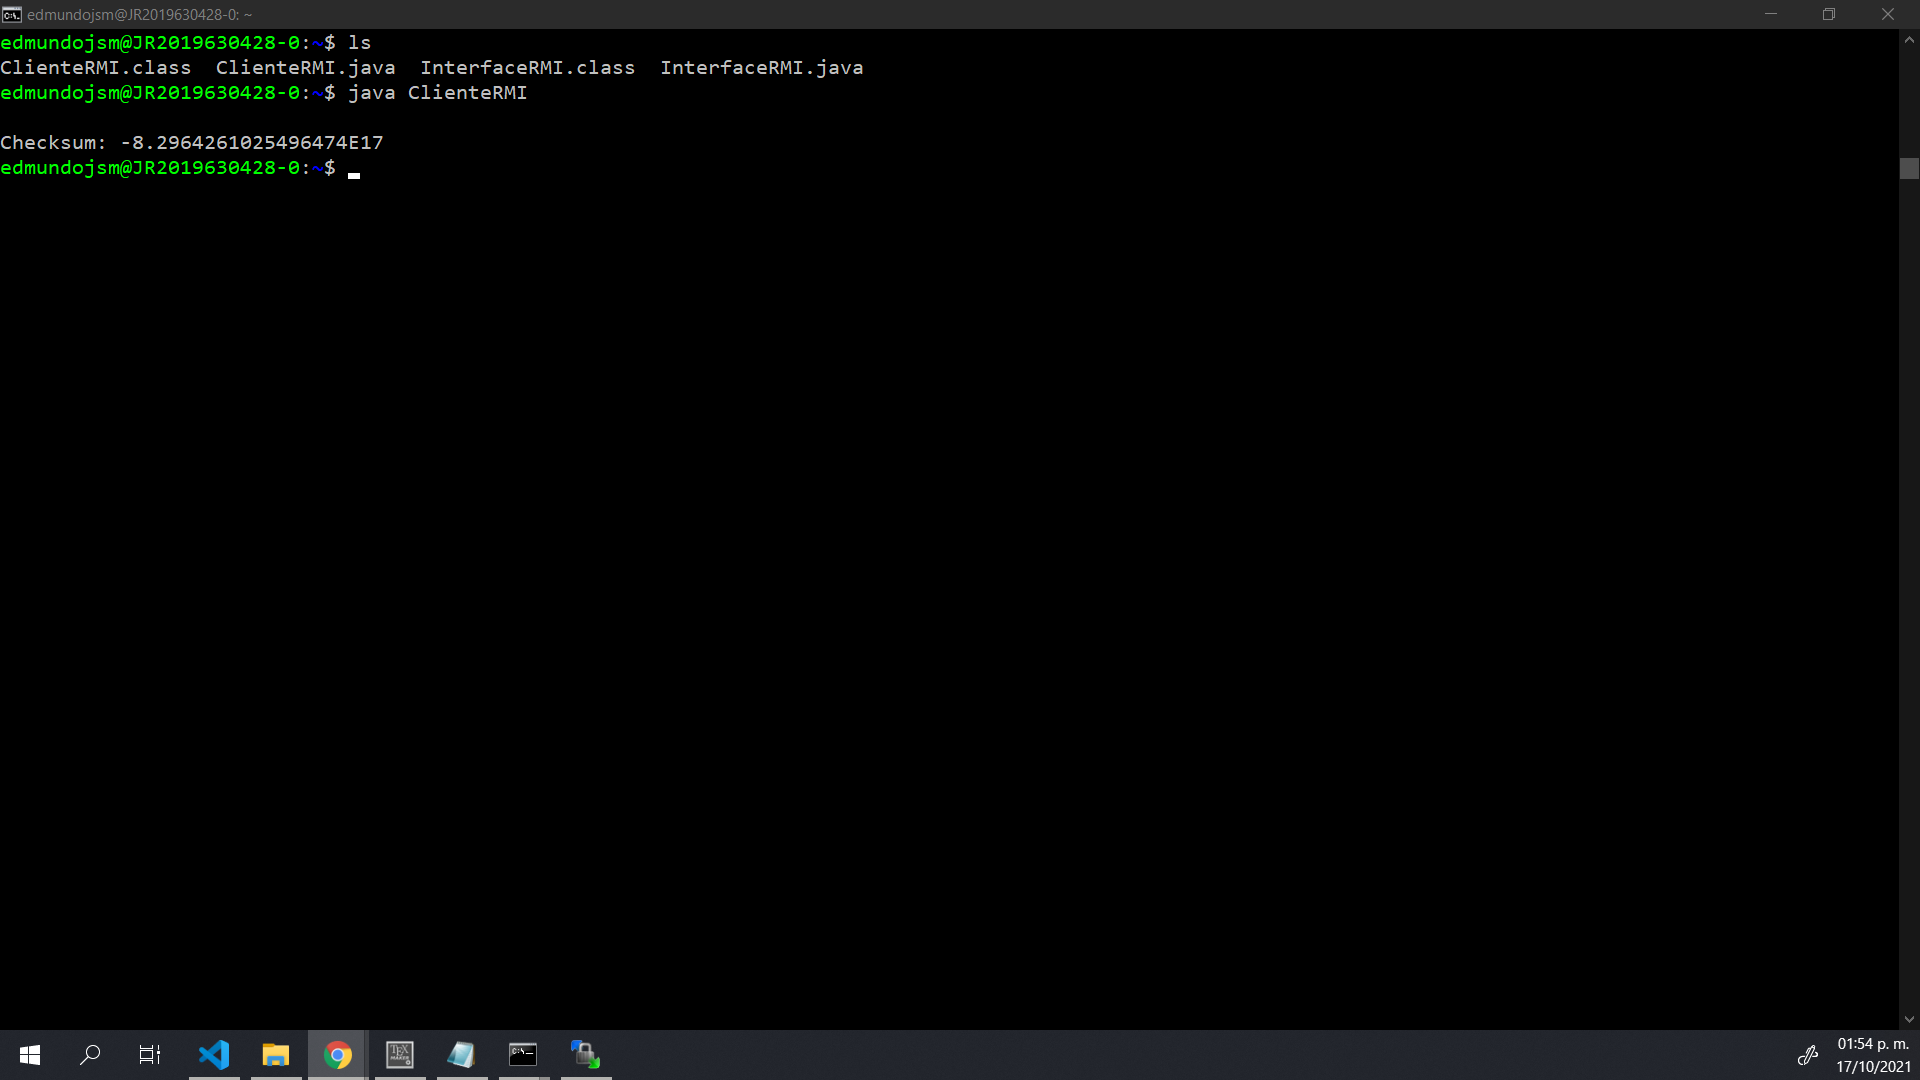
\includegraphics[scale=0.34]{resources/resultado3000.png}
			\caption{Valor de checksum para N=3000.}\label{fig:picture}
		\end{figure}
		Como vemos solo se nos despliega el valor del checksum de la matriz C, que es como se nos pide en la tarea.

	\section{Conclusiones}
	En esta practica implementamos un programa similar a la de la tarea 3, pero en esta ocasión utilizamos Java RMI. Es mucho mas sencillo hacerlo de esta forma ya que el envió de los pedazos de las matrices no nos hes relevante ya que ahora invocamos métodos de manera remota. Para hacer las pruebas creamos 4 maquinas virtuales de Ubuntu Server, en Microsoft Azure. En este caso la implementación de las maquinas es muy sencilla y la conexión a través de ssh facilita mucho las cosas, ademas de que usando WinSCP nos facilita aun mas el paso de los archivos ya que es una forma muy visual el paso de los archivos de la maquina local con las maquinas virtuales. Finalmente me pareció interesante este forma de usar el computo distribuido, ya que nos da una facilidad y agilidad al implementar este tipo de programas.
\end{document}
